% this file demonstrates the use of the NRELreport style file.

% ---------------
% PREAMBLE
% ---------------
\documentclass[tagged]{NRELreport}
%\documentclass[tagged,10pt]{NRELarticle}
\usepackage{hyperref}
\usepackage{tabularx}
\usepackage{units}


% -----------------------------------
\addbibresource{offshore.bib}
% -----------------------------------
% DOCUMENT PROPERTIES
% -----------------------------------
\title{FloatingSE Documentation}
\author{Garrett Barter, PhD}
\date{March 30, 2018}
% -------------------------------------
% CUSTOMIZATIONS
% -------------------------------------

\newcommand{\mytt}[1]{\texttt{\scriptsize #1}}
\newcommand{\mbb}[1]{\mathbb{#1}}
\newcommand{\mbf}[1]{\mathbf{#1}}
\newcommand{\sbf}[1]{\boldsymbol{#1}}
\newcommand{\mcal}[1]{\mathcal{#1}}
% 'st' 'nd' 'rd' 'th' superscripts for numbers
\newcommand{\first}{\raise.5ex\hbox{\small st}}
\newcommand{\second}{\raise.5ex\hbox{\small nd}}
\newcommand{\third}{\raise.5ex\hbox{\small rd}}
\newcommand{\fourth}{\raise.5ex\hbox{\small th}}
\renewcommand{\th}{\raise.5ex\hbox{\tiny th}}

% -------------------------------------
% DOCUMENT STARTS HERE
% -------------------------------------
\lstset{language=Python,columns=fullflexible,keepspaces=true,breaklines=true,basicstyle=\scriptsize\ttfamily,mathescape=true,aboveskip=-6pt,belowskip=0pt}
\setcounter{tocdepth}{1}
\begin{document}

\frontmatter
%\chapter*{Acknowledgements}
The authors thank the following individuals for their thoughtful
reviews, commentary, and suggestions: Daniel Beals, Rick Damiani, Alana
Duerr, Katherine Dykes, Patrick Gilman, Jason Jonkman, Eric Lantz,
Philipp Mucha, Gary Norton, Senu Sirnivas, Richard Tusing.

This work was supported by the U.S. Department of Energy (DOE) under
Contract Number DE-AC36-08GO28308 with NREL. Funding for the work was
provided by the DOE Office of Energy Efficiency and Renewable Energy,
Wind Energy Technologies Office.

% \input{executive_summary}

\mainmatter
\tableofcontents \newpage
\listoffigures
\listoftables

\newpage
\chapter{Introduction}
\label{sec:intro}
The complexity of the physics, economics, logistics, and operation of a
floating offshore wind turbine makes it well suited to systems-focused
solutions.  \textit{FloatingSE} is the floating substructure cost and
sizing module for NREL's Wind-Plant Integrated System Design and
Engineering Model (WISDEM) tool.  WISDEM is a set of integrated modules
that creates a virtual, vertically integrated wind plant. The models use
engineering principles for conceptual design and preliminary analysis,
and link to financial modules for LCOE estimation.

The WISDEM modules, including \textit{FloatingSE}, are built around the
OpenMDAO library, an open-source high-performance computing platform for
systems analysis and multidisciplinary optimization, written in Python
\citep{openmdao}.  Due to the structure of OpenMDAO, and modular design
of WISDEM, individual modules can be exercised individually or in unison
for turbine or plant level studies.  This feature also applies to
\textit{FloatingSE}, in that module-specific optimizations of a floating
substructure and its anchoring and mooring systems can be executed while
treating the rest of the turbine, plant, and operational strategy as
static.  Alternatively, \textit{FloatingSE} can be linked to other
WISDEM modules to execute turbine-level and/or plant-level tradeoff and
optimization studies.

This document serves as both a User Manual and Theory Guide for
\textit{FloatingSE}.  An overview of the package contents is in Section
\ref{sec:package} and substructure geometry parameterization in Section
\ref{sec:geom}.  With this foundation, the underlying theory of
\textit{FloatingSE's} methodology is explained in Section
\ref{sec:theory}.  This helps to understand the analysis execution flow
described in Section \ref{sec:exec} and the setup of design variables
and constraints for optimization problems in Section \ref{sec:opt}.
Finally, some discussion of how \textit{FloatingSE} can be linked to
other WISDEM modules via a high-level OpenMDAO Group is described in
Section \ref{sec:other}.

\chapter{Package Documentation}
\label{sec:package}
The open-source GitHub repository for \textit{FloatingSE} is located at
\url{https://github.com/WISDEM/FloatingSE}.  \textit{FloatingSE} is one of many
modules in the larger WISDEM project and developed primarily by
engineers at the National Renewable Energy Laboratory (NREL).

\section{Package Files}
The files that comprise the \textit{FloatingSE} package are found in the
\texttt{src/floatingse} directory in accordance with standard Python
package conventions.  In addition to the individual files that comprise the package, there are
also unit tests that probe the behavior of individual functions.  These
are located in the \texttt{test} sub-directory.  A summary of all
package files is included in Table \ref{tbl:package}.

\begin{table}[htbp] \begin{center}
    \caption{File contents of the \texttt{src/floatingse} Python package
      within \textit{FloatingSE}.}
    \label{tbl:package}
{\footnotesize
  \begin{tabularx}{\linewidth}{ l l X } \hline
    \textbf{File name} & \textbf{Unit test file} & \textbf{Description} \\ \hline \hline
\mytt{\_\_init\_\_.py} && Generic python package file.\\
\mytt{column.py} & \mytt{column\_PyU.py} & OpenMDAO Components and Group calculating
  mass, buoyancy, and static stability of vertical frustum columns.\\
\mytt{floating.py} && Top level \textit{FloatingSE} OpenMDAO Group.\\
\mytt{floatingInstance.py} && Parent class controlling
  optimization drivers, constraints, and visualization. \\
\mytt{floating\_loading.py} & \mytt{floating\_loading\_PyU.py} &OpenMDAO Components and Group for
  Frame3DD analysis of complete turbine structure and final summation of
  mass and displacement.\\
\mytt{mapMooring.py} & \mytt{mapMooring\_PyU.py} &Mooring analysis.\\
\mytt{semiInstance.py} && Semisubmersible example implementing
  OC4 design parameters, optimization, and visualization.\\
\mytt{sparInstance.py} && Spar example implementing OC3 design
  parameters, optimization, and visualization.\\
\mytt{substructure.py} & \mytt{substructure\_PyU.py} &Final buoyancy and stability checks of
  the substructure.\\
&\mytt{package\_PyU.py} & Convenience aggregator of all unit test files.\\
\hline \end{tabularx}
}
\end{center} \end{table}

\section{Dependencies}
\subsection{Python Dependencies}
The \textit{FloatingSE} directly loads python modules from NumPy, SciPy,
OpenMDAO, and other WISDEM modules.  Each of these packages have
dependencies in their own right.  For visualization, there are optional
calls to Matplotlib and Mayavi.  All of the python dependencies are free
and open-source.

\subsection{WISDEM Dependencies}
The basic functioning of \textit{FloatingSE} relies heavily on \textit{CommonSE}, another
WISDEM module that has general utilities applicable across the WISDEM
suite.  To do a structural analysis on the entire floating turbine
structure, some OpenMDAO Components from \textit{TowerSE} are also called
directly.  In turn, other utilities managed within WISDEM are also
called, such as \textit{Akima} (for differentiable splines), and \textit{pyFrame3DD} (for
structural analysis).  Note that for these other WISDEM modules,
additional Python packages are required, as well as C and Fortran compilers.

\chapter{Geometry}
\label{sec:geom}
This section describes the variables and methods used to parameterize
the substructure geometry in \textit{FloatingSE}.  Typically,
substructure designs have fallen into three classical regimes, which are
shown in Figure \ref{fig:archetype}, each of which attains static stability
through different physical mechanisms.  A spar derives its stability from a
deep drafted ballast.  A semisubmersible derives its stability from
distributed waterplane area, achieved with offset columns spread evenly
around a main column or central point.  A tension leg platform (TLP) uses taut
mooring lines for its stability.

\begin{figure}[htbp]
  \begin{center}
    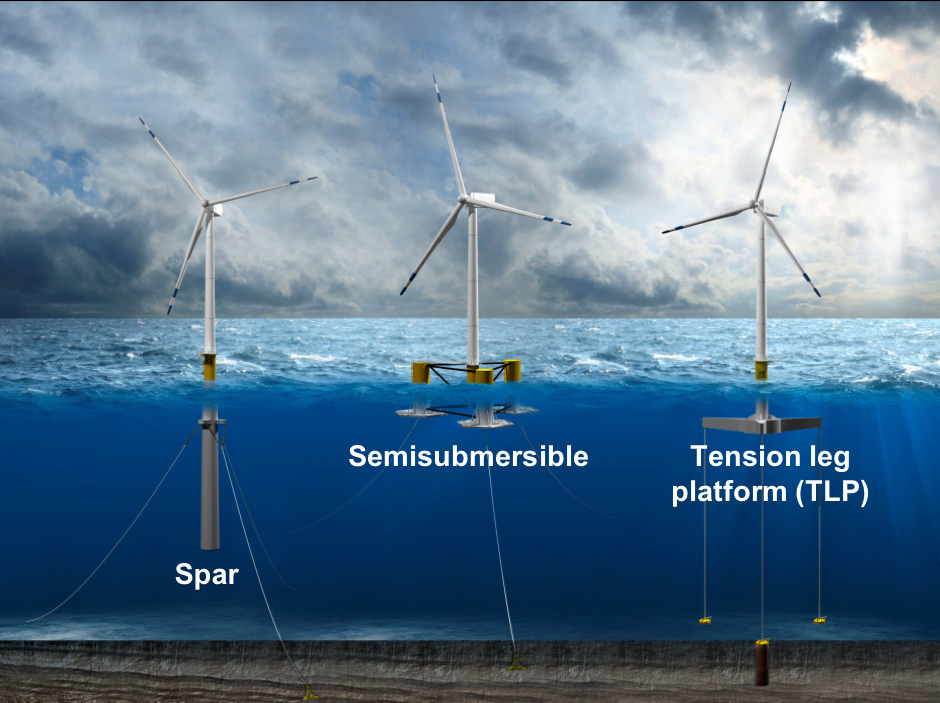
\includegraphics[width=3.75in]{figs/archetypes.pdf}
    \caption{Three classical designs for floating turbine substructures.}
    \label{fig:archetype}
  \end{center}
\end{figure}

Similar to \citet{karimi2017}, care was taken to parameterize the
substructure in a general manner, so as to be able to use the same set
of design variables to describe spars, semisubmersibles, TLPs, and
hybrids of those archetypes.  The intent is that this modular approach
to substructure definition will enable rapid analysis of the majority of
designs currently proposed by the floating wind development community,
whether classical or novel in nature.  Furthermore, generalizing the
substructure definition also empowers the optimization algorithm to
search a broad tradespace more efficiently by moving fluidly from one
region to another.

With that intent in mind, the general configuration of a spar-type
substructure is shown in Figure \ref{fig:diagram}, with nomenclature
borrowed from the field of naval architecture.  A semisubmersible
configuration would have a similar diagram, but with multiple offset
columns connected with pontoon elements.  A TLP might look similar to a
spar or semisubmersible, with taut mooring lines instead of the catenary
ones shown.

\begin{figure}[htb]
  \begin{center}
    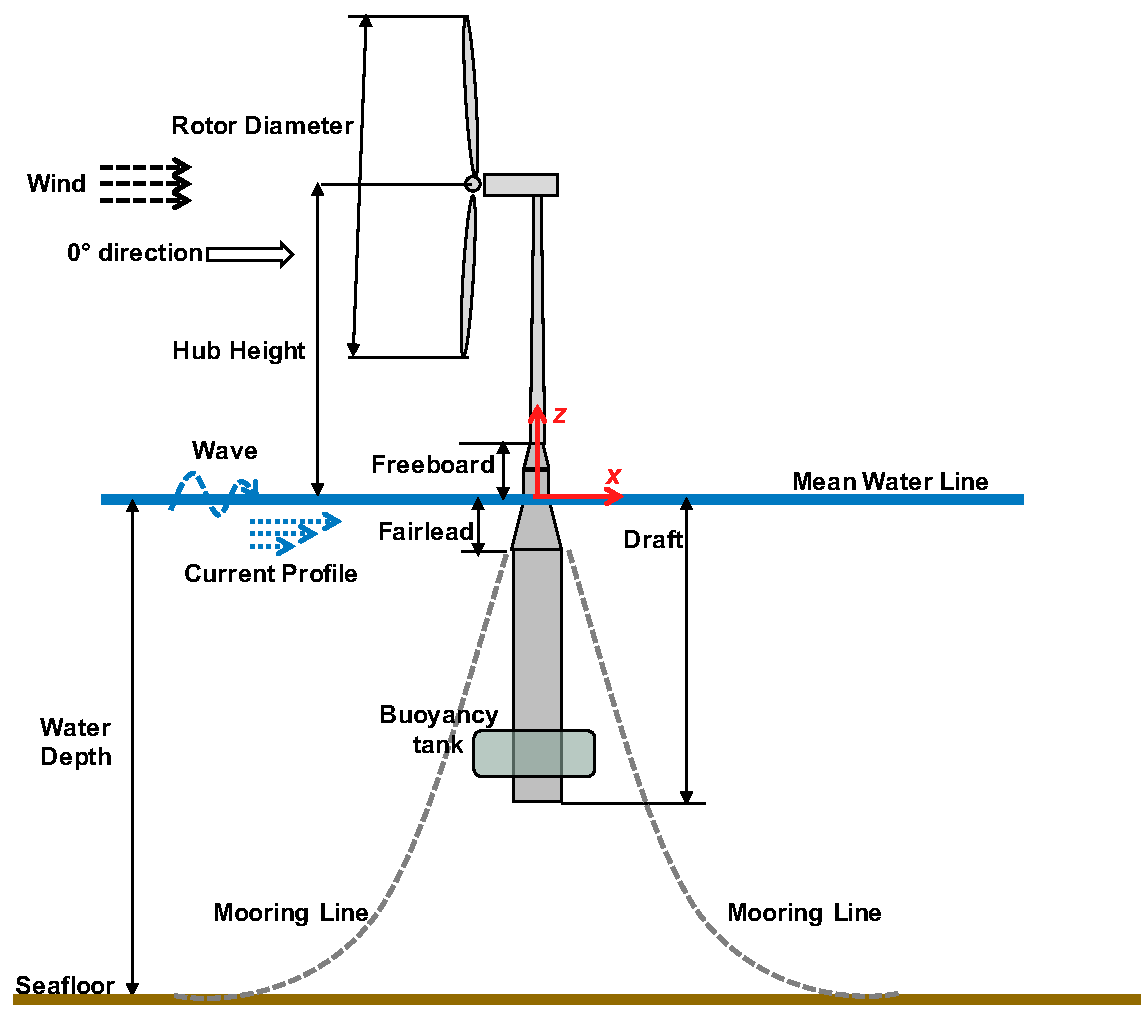
\includegraphics[width=5in]{figs/diagram.pdf}
    \caption{Geometry parameterization with common wind turbine and
      naval architecture conventions.}
    \label{fig:diagram}
  \end{center}
\end{figure}

\section{Tapered Cylinders (Vertical Frustums)}
A number of typical floating substructure designs, such as the spar or
semisubmersible, contain vertically oriented columns.  In
\textit{FloatingSE}, these columns are
assumed to have a circular cross-section making them, formally, vertical
frustums.  These frustums are assumed to be ring-stiffened to support
the buckling loads inherent in a submerged support structure.  The
number of columns, their geometry, and the ring stiffeners are
parameterized in the \textit{FloatingSE} module according to the
diagrams in Figures \ref{fig:diagram} and \ref{fig:column}.  The main
column is assumed to be centered at $(x=0, y=0)$, directly underneath the
turbine tower (note that off-centered turbines are not yet supported).
Other columns are referred to as \textit{offset} columns, and are
assumed to be evenly spread around the main column.  The material of the
vertical columns is currently assumed to be ASTM 992 steel.
Future developments will include the option to select one of multiple
material options for each section in each cylinder.

\begin{figure}[htb]
  \begin{subfigure}[b]{0.38\linewidth}
    \centering 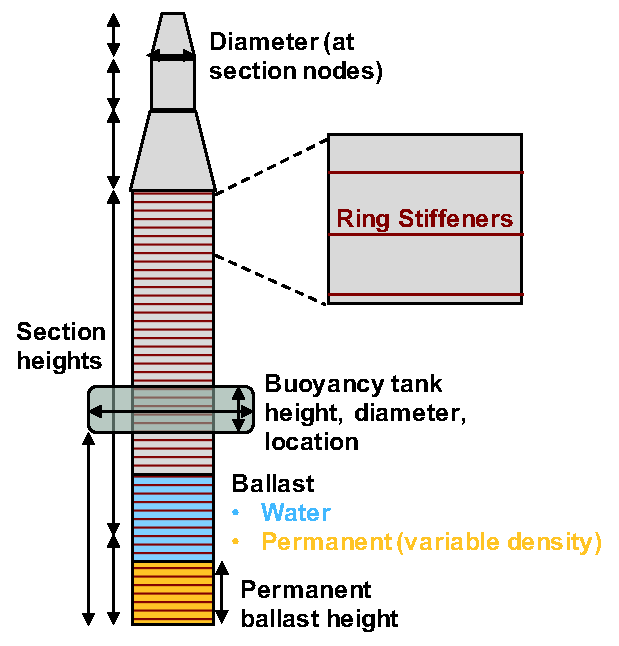
\includegraphics[width=2.2in]{figs/colGeom.pdf}
    \caption{Vertical column of frustums}
  \end{subfigure}
  \begin{subfigure}[b]{0.29\linewidth}
    \centering 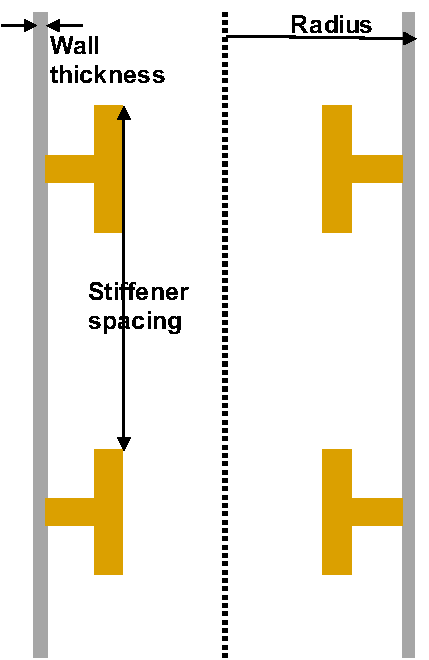
\includegraphics[width=1.8in]{figs/stiffenerCut.pdf}
    \caption{Vertical cross-section}
  \end{subfigure}
  \begin{subfigure}[b]{0.29\linewidth}
    \centering 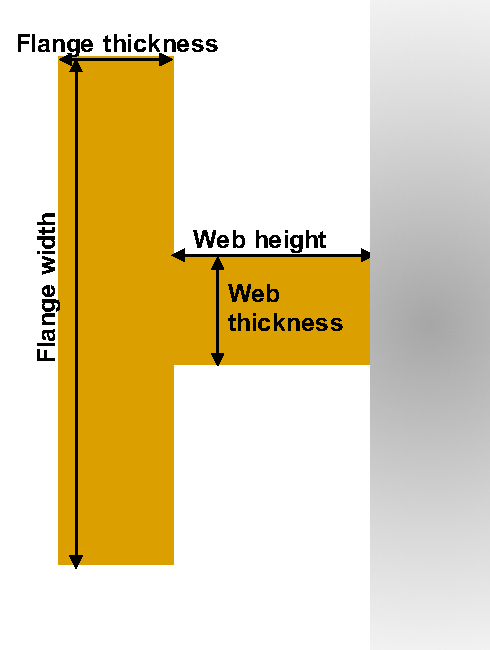
\includegraphics[width=1.8in]{figs/stiffenerZoom.pdf}
    \caption{Ring stiffener geometry}
  \end{subfigure}
  \caption{Vertical frustum geometry parameterization.}
  \label{fig:column}
\end{figure}

The variables that set the geometry of the main and offset columns are listed in Table \ref{tbl:main.ar}.  Two
additional variables are also included that describe the placement of
the offset columns within the substructure configuration.
%
\begin{table}[htbp] \begin{center}
    \caption{Variables specifying the main.column geometry within \textit{FloatingSE}.}
    \label{tbl:main.ar}
{\footnotesize
  \begin{tabular}{ l l c l } \hline
    \textbf{Variable} & \textbf{Type} & \textbf{Units} & \textbf{Description} \\
    \mytt{main\_section\_height} & Float array ($n_s$) & $m$& Height of each section \\
    \mytt{main\_outer\_diameter} & Float array ($n_s+1$) & $m$&Diameter at each section node (linear lofting between) \\
    \mytt{main\_wall\_thickness} & Float array ($n_s+1$) & $m$&Wall thickness at each section node (linear lofting between) \\
    \mytt{main\_freeboard} & Float scalar & $m$&Design height above waterline \\
    \mytt{offset\_section\_height} & Float array ($n_s$) & $m$& Height of each section \\
    \mytt{offset\_outer\_diameter} & Float array ($n_s+1$) & $m$&Diameter at each section node (linear lofting between) \\
    \mytt{offset\_wall\_thickness} & Float array ($n_s+1$) & $m$&Wall thickness at each section node (linear lofting between) \\
    \mytt{offset\_freeboard} & Float scalar & $m$&Design height above waterline \\
    \mytt{number\_of\_offset\_columns} & Integer scalar && Number of offset columns in substructure (for spar set to 0)\\
    \mytt{radius\_to\_offset\_column} & Float scalar &$m$& Centerline of main.column to centerline of offset column\\
  \hline \end{tabular}
}
\end{center} \end{table}

\subsection{Discretization}
To allow for varying geometry parameters along the length of
substructure columns, the larger components are divided into sections.
The user may specify the number of overall sections, $n_s$ and the
geometry of each section.  Some of the geometry parameters are tied to
the nodes that bracket each section, such as column diameter and wall
thickness, with linear variation between each node.  Other parameters
are considered constant within each section, such as the spacing between
ring stiffeners.  The number of sections should resemble the physical
number of cans or sections used in the manufacturing of the real
article.

\subsection{Stiffeners}
The ring stiffener geometry is depicted in Figure \ref{fig:column}b--c
with geometry variables listed in Table \ref{tbl:stiffvar}
%
\begin{table}[htbp] \begin{center}
    \caption{Variables specifying the stiffener geometry within \textit{FloatingSE}.}
    \label{tbl:stiffvar}
{\footnotesize
  \begin{tabular}{ l l c l } \hline
    \textbf{Variable} & \textbf{Type} & \textbf{Units} & \textbf{Description} \\
    \mytt{main\_stiffener\_web\_height} & Float array ($n_s$) &$m$& Stiffener web height for each section \\
    \mytt{main\_stiffener\_web\_thickness} & Float array ($n_s$) &$m$& Stiffener web thickness for each section\\
    \mytt{main\_stiffener\_flange\_width} & Float array ($n_s$) &$m$& Stiffener flange width for each section\\
    \mytt{main\_stiffener\_flange\_thickness} & Float array ($n_s$) &$m$& Stiffener flange thickness for each section\\
    \mytt{main\_stiffener\_spacing} & Float array ($n_s$) &$m$& Stiffener spacing for each section\\
  \hline \end{tabular}
}
\end{center} \end{table}

\subsection{Material Properties}
The material of the vertical columns is currently assumed to uniformly
be ASTM 992 steel.  Future developments will include the option to
select one of multiple material options for each section in each
cylinder.  Currently, to globally change to a different material, use
the variables listed in Table \ref{tbl:materialvar}.
%
\begin{table}[htbp] \begin{center}
    \caption{Variables specifying the material properties within \textit{FloatingSE}.}
    \label{tbl:materialvar}
{\footnotesize
  \begin{tabular}{ l l c l } \hline
    \textbf{Variable} & \textbf{Type} & \textbf{Units} & \textbf{Description} \\
    \mytt{material\_density} & Float scalar & $kg/m^3$& Mass density (assumed steel) \\
    \mytt{E} & Float scalar & $N/m^2$& Young's modulus (of elasticity) \\
    \mytt{G} & Float scalar & $N/m^2$& Shear modulus \\
    \mytt{yield\_stress} & Float scalar & $N/m^2$& Elastic yield stress \\
    \mytt{nu} & Float scalar && Poisson's ratio ($\nu$)\\
  \hline \end{tabular}
}
\end{center} \end{table}

\subsection{Ballast}
Stability of substructure columns with long drafts can be enhanced by
placing heavy ballast, such as magnetite iron ore, at their bottom
sections.  The user can specify the density of the permanent ballast
added and the height of the ballast extent within the column. The variables that govern the implementation of the
permanent ballast and bulkhead nodes are listed in Table
\ref{tbl:ballastvar}.  Variable
ballast, as opposed to permanent ballast, is water that is added or
removed above the permanent ballast to achieve neutral buoyancy as the
operating conditions of the turbine change.  A discussion of variable
water balance in the model is found in Section \ref{sec:static}.
%
\begin{table}[htbp] \begin{center}
    \caption{Variables specifying the ballast and bulkheads within \textit{FloatingSE}.}
    \label{tbl:ballastvar}
{\footnotesize
  \begin{tabular}{ l l c l } \hline
    \textbf{Variable} & \textbf{Type} & \textbf{Units} & \textbf{Description} \\
    \mytt{permanent\_ballast\_density} & Float scalar & $kg/m^3$& Mass density of ballast material \\
    \mytt{main\_permanent\_ballast\_height} & Float scalar & $m$& Height above keel for permanent ballast \\
    \mytt{main\_bulkhead\_thickness} & Float vector ($n_s+1$) &$m$& Internal bulkhead thicknesses at section interfaces\\
    \mytt{offset\_permanent\_ballast\_height} & Float scalar & $m$& Height above keel for permanent ballast \\
    \mytt{offset\_bulkhead\_thickness} & Float vector ($n_s+1$) &$m$& Internal bulkhead thicknesses at section interfaces\\
  \hline \end{tabular}
}
\end{center} \end{table}


\subsection{Buoyancy Tanks (and Heave Plates)}
Buoyancy tanks are modeled as a collar around the column and are not
subject the same taper or connectivity constraints as the frustum
sections.  They therefore offer added buoyancy without incurring as much
structural mass or cost.  Moreover, they can also serve to augment the
heave added mass like a plate.  The variables that govern
their configuration are listed in Table \ref{tbl:buoyheave}.  In addition to their diameter and
height, the user can adjust the location of the buoyancy tank from the
column base to the top. Buoyancy tanks can be added to either the main
and/or offset columns.
%
\begin{table}[htbp] \begin{center}
    \caption{Variables specifying the buoyancy tank geometry within \textit{FloatingSE}.}
    \label{tbl:buoyheave}
{\footnotesize
  \begin{tabular}{ l l c l } \hline
    \textbf{Variable} & \textbf{Type} & \textbf{Units} & \textbf{Description} \\
    \mytt{main\_buoyancy\_tank\_diameter} & Float scalar & $m$& Diameter of buoyancy tank / heave plate on main.column\\
    \mytt{main\_buoyancy\_tank\_height} & Float scalar & $m$& Height of buoyancy tank / heave plate on main.column\\
    \mytt{main\_buoyancy\_tank\_location} & Float scalar & & Location of buoyancy tank along main.column (0 for bottom, 1 for top)\\
    \mytt{offset\_buoyancy\_tank\_diameter} & Float scalar & $m$& Diameter of buoyancy tank / heave plate on offset column\\
    \mytt{offset\_buoyancy\_tank\_height} & Float scalar & $m$& Height of buoyancy tank / heave plate on offset column\\
    \mytt{offset\_buoyancy\_tank\_location} & Float scalar & & Location of buoyancy tank along offliary column (0 for bottom, 1 for top)\\
  \hline \end{tabular}
}
\end{center} \end{table}


\section{Pontoons and Support Structure}
Many substructure designs include the use of pontoons that form a truss
to connect the different components, usually columns, together.  In this
model, all of the pontoons are assumed to have the identical thin-walled
tube cross section and made of the same material as the rest of the
substructure.  The truss configuration and the parameterization of the
pontoon elements is based on the members shown in Figure
\ref{fig:pontoon} with lettered labels.  The members are broken out into
the upper and lower rings connecting the offset columns ($B$ and $D$,
respectively), the upper and lower main-to-offset connections ($A$ and
$C$, respectively), the lower-base to upper-offset cross members ($E$),
and the V-shaped cross members between offset columns ($F$). The
variables that drive this parameterization are listed in Table
\ref{tbl:trussvar}.
%
\begin{figure}[htb]
  \begin{center}
    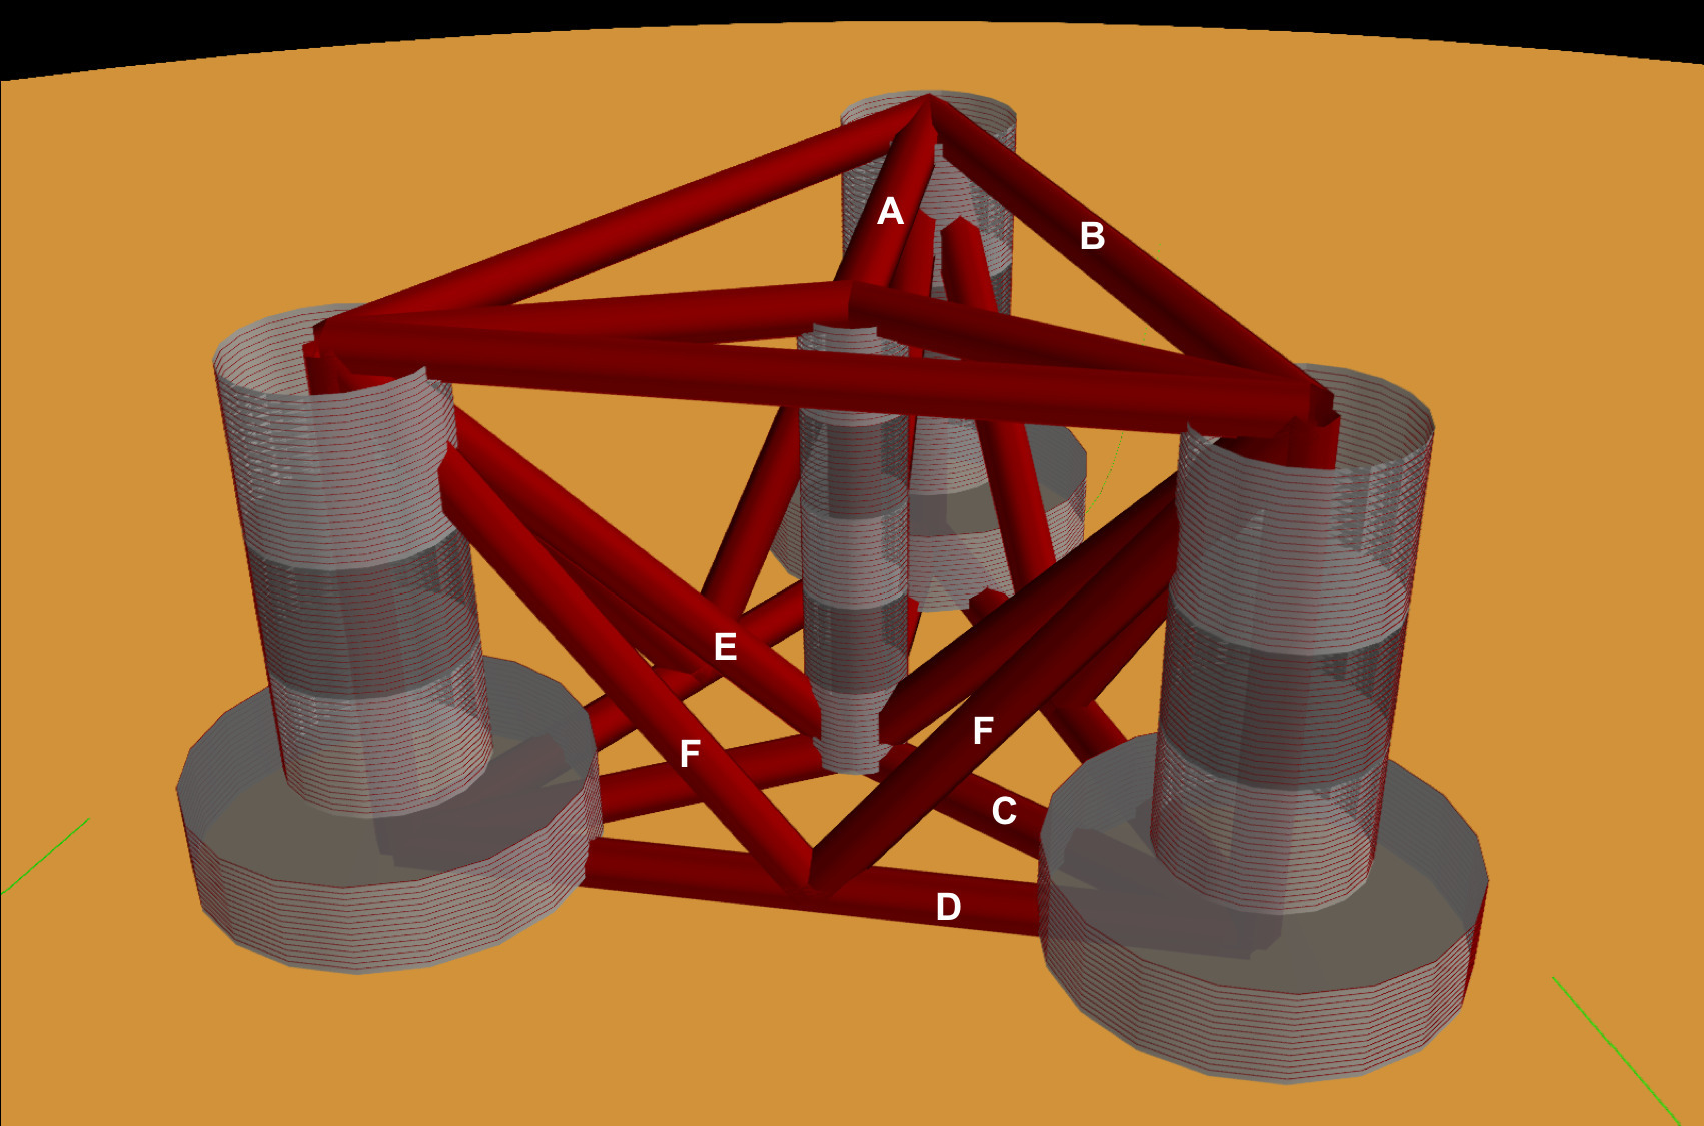
\includegraphics[width=4.5in]{figs/semi.pdf}
    \caption{Parameterization of truss elements in substructure.}
    \label{fig:pontoon}
  \end{center}
\end{figure}
%
\begin{table}[htbp] \begin{center}
    \caption{Variables specifying the pontoon and truss geometry within \textit{FloatingSE}.}
    \label{tbl:trussvar}
{\footnotesize
  \begin{tabular}{ l l c c l } \hline
    \textbf{Variable} & \textbf{Type} & \textbf{Figure \ref{fig:pontoon}} & \textbf{Units} & \textbf{Description} \\
    \mytt{pontoon\_outer\_diameter} & Float scalar & & $m$& Diameter of all pontoon/truss elements \\
    \mytt{pontoon\_wall\_thickness} & Float scalar & & $m$& Thickness of all pontoon/truss elements \\
    \mytt{main\_pontoon\_attach\_lower} & Float scalar & & $m$& Lower z-coordinate on main.where truss attaches \\
    \mytt{main\_pontoon\_attach\_upper} & Float scalar & & $m$& Upper z-coordinate on main.where truss attaches \\
    \mytt{upper\_attachment\_pontoons} & Boolean & A && Upper main.to-offset connecting pontoons\\
    \mytt{lower\_attachment\_pontoons} & Boolean & C && Lower main.to-offset connecting pontoons\\
    \mytt{cross\_attachment\_pontoons} & Boolean & E && Lower-Upper main.to-offset connecting cross braces\\
    \mytt{upper\_ring\_pontoons} & Boolean & B && Upper ring of pontoons connecting offset columns\\
    \mytt{lower\_ring\_pontoons} & Boolean & D && Lower ring of pontoons connecting offset columns\\
    \mytt{outer\_cross\_pontoons} & Boolean & F && Auxiliary ring connecting V-cross braces\\
  \hline \end{tabular}
}
\end{center} \end{table}


\section{Mooring Lines}
The mooring system is described by the number of lines, their geometry,
and their interface to the substructure.  The mooring diameter is set by
the user and determines the breaking load and stiffness of the chain,
via correlation, described in Section \ref{sec:theory}.  The mooring
lines attach to the substructure at the \textit{fairlead} distance below
the water plane, as shown in Figure \ref{fig:diagram}.  The lines can
attach directly to a substructure column or at a some offset from the
outer shell.  Note that bridle connections are not yet implemented in
the model.  The mooring lines attach to the sea floor at a variable
distance, the anchor radius, from the substructure centerline, also set
by the user.

By default, the mooring system is assumed to use a steel chain with drag
embedment anchors. Other mooring available for selection are nylon,
polyester, steel wire rope (IWRC) and fiber-core wire rope.  The only
alternative anchor type is currently suction pile anchors, but there are
plans to include gravity anchors as well.  The standard configuration
for TLPs is the use of taut nylon mooring lines with suction-pile
anchors.  The variables that control the mooring system properties are
listed in Table \ref{tbl:moorvar}.
%
\begin{table}[htbp] \begin{center}
    \caption{Variables specifying the mooring system within \textit{FloatingSE}.}
    \label{tbl:moorvar}
{\footnotesize
  \begin{tabular}{ l l c l } \hline
    \textbf{Variable} & \textbf{Type} & \textbf{Units} & \textbf{Description} \\
    \mytt{number\_of\_mooring\_connections} & Integer scalar && Number
    of evenly spaced mooring connection points\\
    \mytt{mooring\_lines\_per\_connection} & Integer scalar && Number of mooring lines at each connection point\\
    \mytt{mooring\_diameter} & Float scalar & $m$& Diameter of mooring line/chain \\
    \mytt{mooring\_line\_length} & Float scalar &$m$& Total unstretched line length of mooring line\\
    \mytt{fairlead\_location} & Float scalar && Fractional length from column bottom to mooring line attachment \\
    \mytt{fairlead\_offset\_from\_shell} & Float scalar & $m$ & Offset from shell surface for mooring attachment \\
    \mytt{anchor\_radius} & Float scalar & $m$& Distance from centerline to sea floor landing \\
    \mytt{mooring\_type} & Enumerated & & Options are CHAIN, NYLON, POLYESTER, FIBER, or IWRC\\
    \mytt{anchor\_type} & Enumerated & & Options are SUCTIONPILE or DRAGEMBEDMENT\\
  \hline \end{tabular}
}
\end{center} \end{table}



\section{Mass and Cost Scaling}
The mass of all components in the modeled substructure is captured
through calculation of each components' volume and multiplying by its material
density.  This applies to the frustum shells, the ring stiffeners, the
permanent ballast, the pontoons, and the mooring lines.
However, the model also acknowledges that the modeled substructure is
merely an approximation of an actual substructure and various secondary
elements are not captured.  These include ladders, walkways, handles,
finishing, paint, wiring, etc.  To account for these features en masse,
multipliers of component masses are offered as parameters for the user
as well.  Capital cost for all substructure components except the
mooring system is assumed to be a linear scaling of the components
masses.  For the mooring system, cost is dependent on the tension
carrying capacity of the line, which itself is an empirical function of
the diameter.  Default values for all mass and cost scaling factors are
found in Table \ref{tbl:factors}.  Cost factors are especially difficult to
estimate given the proprietary nature of commercial cost data, so
cost rates and estimates should be considered notional.
%
\begin{table}[htbp] \begin{center}
    \caption{Variables specifying the mass and cost scaling within \textit{FloatingSE}.}
    \label{tbl:factors}
{\footnotesize
  \begin{tabular}{ l l c r l } \hline
    \textbf{Variable} & \textbf{Type} & \textbf{Units} & \textbf{Default} & \textbf{Description} \\
    \mytt{bulkhead\_mass\_factor}     & Float scalar     &&1.0& Scaling for unaccounted bulkhead mass\\
    \mytt{ring\_mass\_factor}         & Float scalar     &&1.0& Scaling for unaccounted stiffener mass\\
    \mytt{shell\_mass\_factor}        & Float scalar     &&1.0& Scaling for unaccounted shell mass\\
    \mytt{column\_mass\_factor}       & Float scalar    &&1.05& Scaling for unaccounted column mass\\
    \mytt{outfitting\_mass\_fraction} & Float scalar    &&0.06& Fraction of additional outfitting mass for each column\\
    \mytt{ballast\_cost\_rate}        & Float scalar   & $USD/kg$&100& Cost factor for ballast mass \\
    \mytt{tapered\_col\_cost\_rate}    & Float scalar  & $USD/kg$&4,720& Cost factor for column mass \\
    \mytt{outfitting\_cost\_rate}     & Float scalar  & $USD/kg$&6,980& Cost factor for outfitting mass \\
    \mytt{mooring\_cost\_rate}        & Float scalar     &
    $USD/kg$&depends& Mooring cost factor (depends on diam and material) \\
    \mytt{pontoon\_cost\_rate}        & Float scalar   & $USD/kg$&6.5& Cost factor for pontoons \\
  \hline \end{tabular}
}
\end{center} \end{table}

\chapter{Theory}
\label{sec:theory}

\section{Design Load Cases}
The user must specify the metocean conditions that drive the wind and
wave loads upon the floating substructure.  Ideally, multiple metocean
conditions would be used for design optimization, many of which have
already been codified \citep{iec2009}.  This includes standard operating
conditions that determine fatigue loads, maximum allowable operating
conditions (e.g. max thrust), maximum survivable conditions, and likely
others that bound a design.  As of this writing, \textit{FloatingSE}
only supports execution and optimization around a single metocean
condition and load case.  Future development will enable optimization
against a vector of load cases, likely those used in code standards.

\section{Load Path}
Similar to the assumptions in \textit{JacketSE}, as stated by
\citep{JacketSE}, the primary simplification in \textit{FloatingSE} is
the treatment of all loads as pseudo-static. This approximation reduces
computational time and resources, since an accurate calculation of
dynamic loads requires more sophisticated numerical tools and
simulations.  Thus, users must exercise care in selecting loads and
safety factors to compensate for the lack of a fully dynamic treatment.
Furthermore, fatigue effects and structural lifetime estimates are also
not currently calculated, but could be incorporated in future
developments.  In general though, fatigue loading tends to dominate the
design of joints, flanges, and welds in a design (which are not
prominently featured in \textit{FloatingSE}), whereas overall structural
sizing of the main shell geometry is driven by modal and
buckling-strength requirements (which are prominently featured in
\textit{FloatingSE}).

A floating wind turbine undergoes loading from a number of sources.  The
primary loading source for the tower comes from the aerodynamic loads
induced by the rotor. The substructure must resist the combination of
both rotor loads and hydrodynamics loads, with the latter becoming more
and more important as water depth and wave heights increase.
\textit{FloatingSE}, together with other WISDEM modules, accounts for
these two dominant load sources, as well as the self-loading of gravity
loads.  Other sources of loading, such as installation loads, accidental
loads, vortex-induced vibrations, ice, and seismic loads are ignored.

Aerodynamic and hydrodynamic loads are computed within
\textit{FloatingSE} and \textit{CommonSE}.  Rotor thrust loads are
computed in \textit{RotorSE}, and imputed into \textit{FloatingSE} as
inputs.  Loading over the entire turbine is then assembled within
\textit{FloatinSE} for a structural analysis by Frame3DD (via
\textit{pyFrame3DD}).  Once all member loads and stresses are
determined, compliance checks against international standards are
evaluated and can be used as design constraints during optimization
runs.

\subsection{Wind and Wave Loads}
Wind drag loads are applied to the tower body and the upper part of the
substructure that extends above the waterline.  They are not applied to
connecting truss members that may be part of the substructure geometry.
These drag loads are computed assuming the tower and columns are smooth
circular cross-sections and that the drag coefficient can be selected as
a function of the flow Reynolds number \citep{Roshko}.  The calculations
of the wind and wave loads are provided by multiple modules within
\textit{CommonSE}.

For the tower and portion of the substructure that extends above the
waterline, wind loading arises from the aerodynamic drag on the
structure.  This drag changes with height, since the wind profile and
cross-sectional geometry varies.  WISDEM allows the user to select from
a power-law or logarithmic scaling of wind with height, where the
power-law approximation is given by,
\[
  U_a(z) = U_{ref}\left(\frac{z}{z_{ref}}\right)^{\alpha}\quad,
\]
where $U_a(z)$ is the wind velocity as a function of height, $U_{ref}$ is a
reference wind speed measured at a reference height, $z_{ref}$, and
$\alpha$ is the shear exponent used in the power-law approximation of
wind profiles.  The wind profile then feeds the aerodynamic drag,
Reynolds number, and drag coefficient,
\begin{equation} \label{eqn:drag}
  dF(z) = \frac{1}{2} \rho_a U_a^2(z) d(z) c_d(Re) dz;\qquad
  Re_d = \frac{\rho_a U_a(z) d(z)}{\mu_a}\quad,
\end{equation}
where $Re_d$ is the Reynolds number based on diameter, $\rho_a$ and
$\mu_a$ are the density and viscosity of air, $d(z)$ is the diameter of
the column as a function of height, $c_d$ is the 2-D drag coefficient, and
$dF(z)$ is the force per unit length in the z-direction.

Wave drag loads arise from similar processes, but are computed using
Morison's equation to account for the different fluid properties and
dominant physics relative to air.  Morison's equation is a
semi-empirical expression, as opposed to a model of a specific physical
process, that predicts the total hydrodynamic loads.  It is comprised of
two components, one for viscous drag contributions and another for
inertial effects (which includes incident, diffracted, and radiated wave
effects).  For flow past structures with circular cross sections,
Morison's equation for force per unit length ($dF(z)$) takes the form,
\begin{equation} \label{eqn:morison}
  dF(z) = \frac{\pi d^2(z)}{4} \rho_w C_m \dot{U}_w(z)dz + \frac{1}{2} \rho_w U_w^2(z) d(z) c_d(Re)dz\quad,
\end{equation}
where $C_m$ is the added mass coefficient (assumed to be $C_m=2$),
$U_w(z)$ is the current speed as a function of height, $\dot{U}_w(z)$ is
the acceleration as a function of height, and the Reynolds number is
computed by substituting in the appropriate properties for water,
\[
Re_d = \frac{\rho_w U_w(z) d(z)}{\mu_w}\quad.
\]

To compute Morison's equation, expressions for local fluid velocity and
acceleration are required.  Wave particle velocity (not the same as the bulk
velocity of the wave) is assumed to follow linear (Airy) wave theory
\begin{equation} \label{eqn:Uwave}
U_w(z) = a\omega\frac{\cosh\left[\kappa\left(z + D \right)\right]}{\sinh\left(\kappa D\right)}\cosh\left(\kappa x -
  \omega t\right);
\qquad \omega=\frac{2\pi}{T} = \sqrt{ g \kappa \tanh\left(\kappa
    D\right) } \quad,
\end{equation}
where $\omega$ is the circular frequency, $T$ is the wave period, $a$ is
the wave amplitude (half of the significant wave height), $D$ is the
total water depth, $g$ is the acceleration of gravity, and $\kappa$ is
the wave number numerically computed from the dispersion relationship
given as the last expression in Equation \ref{eqn:Uwave}.  Note that the
horizontal particle velocity varies in time and space (by the
$\kappa x - \omega t$) term.  Thus, the individual particles in the wave
are also accelerating at different rates,
\begin{equation} \label{eqn:Awave}
\dot{U}_w(z) = a\omega^2\frac{\cosh\left[\kappa\left(z + D \right)\right]}{\sinh\left(\kappa D\right)}\sinh\left(\kappa x -
  \omega t\right)\quad.
\end{equation}
For
simplicity, \textit{FloatingSE} only considers the maximum velocity and
acceleration at a given height, and makes a conservative assumption that
they occur concurrently in time and space.  This essentially means ignoring the
$\kappa x - \omega t$ term, since the maximum of any hyperbolic sine or cosine
term is one.



\subsection{Rotor Nacelle Assembly (RNA) Loads}
From a quasi-steady-state point of view, the RNA loads reduce to three
forces and three moments along the main coordinate axes
\citet{JacketSE}. The thrust is the biggest force responsible for the
bending moment distribution along the tower and loads on the
substructure.  There is the additional effect of the gravitational load
caused by the offset of the RNA center of mass from the tower
centerline.  This effect is more pronounced for downwind turbines than
upwind turbines, but is included regardless.

\textit{FloatingSE} does not compute the force and moment components
directly, but rather accepts them as inputs from other WISDEM modules or
from the user directly.  The methodology and fidelity in the RNA loads
calculation are addressed in \textit{RotorSE} and \textit{DriveSE}.


\subsection{Loads Integration and Structural Analysis}
The analysis tool, Frame3DD, is an open-source tool for static and
dynamic structural analysis of 2-D and 3-D frames and trusses with
elastic and geometric stiffness. It computes the static deflections,
reactions, internal element forces, natural frequencies, and modal
shapes using direct stiffness and mass assembly \citep{frame3dd}.  The
WISDEM toolkit developed a python interface, \textit{pyFrame3DD}, to
avoid the use of intermediate input and output text files.  All of the
loads integration happens within Frame3DD, where the whole floating
turbine load path, from the rotor to the keel of the substructure, is
modeled with simple Timoshenko frame elements \citep{timoshenko}.

\subsubsection{Discretization}
Long slender components, such as the tower and substructure columns, are
broken up into a finer discretization than the physical ``cans'' that
they are actually made of.  This finer discretization gives greater
resolution of internal forces and natural frequencies.  Substructure
pontoons are represented as single frame elements.  Frame elements are
described by their cross sectional properties (area, moments of inertia,
modulus of elasticity, and mass density) and starting and ending nodes.
For simple geometries, such as pontoons with tubular cross sections,
these properties are straightforward calculations.  For the turbine
tower, tubular cross section properties are also used, albeit at a finer
discretization.  For substructure columns, which may have permanent or
variable ballast and bulkheads, it is assumed that these extra features
are not load-bearing, so tubular cross section properties are also used.
However, the material mass density of the frame element is scaled to
reflect the true mass of the whole section, including ballast, to ensure
that gravity loads are captured correctly.  Thus, for the tower,
columns, and pontoons, only cylindrical (tubular) cross-sections are
supported for now.  Future development may support other cross-sectional
geometries.  For the tubular cross sections, the critical properties
needed by Frame3DD given user inputs of diameter, $d$, and tube (or
wall) thickness, $t$, are,
\begin{align*}
  \textrm{Outer radius, } r_o &= d/2\\
  \textrm{Inner radius, } r_i &= r_o - t\\
  \textrm{Material area, } A &= \pi \left( r_o^2 - r_i^2 \right)\\
  \textrm{Bending second moment of area, } I_{xx} &= I_{yy} = \frac{\pi}{4}\left( r_o^4 - r_i^4 \right)\\
  \textrm{Torsion second moment of area, } I_{zz} &= J_0 = I_{xx} + I_{yy}\\
  \textrm{Shear area, } A_{s} &= A / \left[ 1.124235 + 0.055610\left(\frac{r_i}{r_o}\right) +
           1.097134\left(\frac{r_i}{r_o}\right)^2 - 0.630057\left(\frac{r_i}{r_o}\right)^3 \right]\\
  \textrm{Bending modulus, } S &= I_{xx} / r_o \\
  \textrm{Torsion modulus (shear constant), } C &= I_{zz} / r_o
\end{align*}
Note that the shear area expression is an empirical relationship as
opposed to an analytical expression.

\begin{figure}[htb]
  \begin{center}
    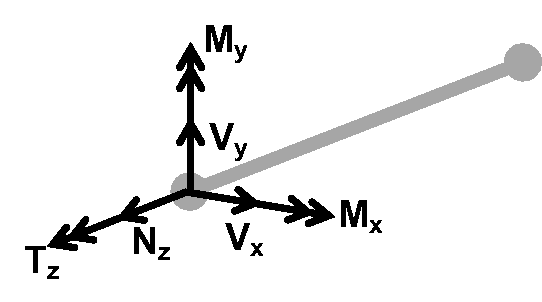
\includegraphics[width=2in]{figs/frameCS.pdf}
    \caption{Coordinate system for frame element forces.}
    \label{fig:frameCS}
  \end{center}
\end{figure}

\subsubsection{Loads}
The forces, moments, and mass properties of the rotor-nacelle assembly
(RNA) are inputs to \textit{FloatingSE} (mass properties are assumed to
be relative to the tower top position).  It assumed that the RNA is a
rigid body with respect to the tower modes and the mass properties,
forces, and moments, are applied to the corresponding node in the model.
The forces along each mooring line are applied upon their connection
point nodes on the structure.  The wind and wave forces per unit length
in Equations \ref{eqn:drag} and \ref{eqn:morison} are applied as
trapezoidally varying loads along the column elements.  Other loads
applied to the structure include the gravity loads, and the buoyancy
acting on the submerged elements.

\subsubsection{Boundary Conditions}
Multiple boundary conditions are applied to the structure.  The mooring
system stiffness matrix (linearized about the neutral position) is
applied at the mooring connection nodes.  However, even with the mooring
stiffness, the finite element analysis would otherwise still regard the
structure as unrestrained and incapable of supporting any static loads.
Thus, in order to successfully compute stress and buckling limits in a
well-posed problem, an additional rigid boundary condition (in all 6
DOF) is imposed at the bottom node of the base column.

\subsubsection{Outputs}
Simulation outputs include mass properties of the structure, member
stresses, and summary forces and moments on the body.  Mass properties
include the total mass of the floating turbine and the mass of the
substructure itself.  The calculations also allow for easy computation
of the center of mass of the structure (not accounting for variable
ballast) and the center of buoyancy (centroid of the submerged volume).
The first two natural frequencies of the structure are also computed to
compare against the range of standard wave frequencies and rotor passing
frequencies (1P and 3P).  Next, the reaction forces and moments at the
boundary mooring load are taken as the total loading on the structure.
These are used later in the static stability calculations to ensure that
the mooring lines provide adequate restoring force and moment.  Finally,
the axial and shear forces are extracted and converted to stresses using
cross-sectional properties for all frame elements.  These element member
loads follow the sign convention in Figure \ref{fig:frameCS},
\begin{align*}
  \sigma_z &= \frac{N_z}{A} - \frac{\sqrt{M_x^2 + M_y^2}}{S}\\
  \tau_{z\theta} &= \frac{T_z}{C} + \frac{\sqrt{V_x^2 + V_y^2}}{A_s}
\end{align*}
where $N$ is the axial force (tension or compression), $T$ is the
torsional moment, $V$ is the shear force, $M$ is the bending moment,
$\sigma_z$ is the axial stress, and $\tau_{z\theta}$ is the shear
stress across axial and hoop principle directions.

Hoop
stress of the tower is estimated from the dynamic pressure of the
wind loads using the Eurocode method.  Hoop stress of the submerged
columns is determined using the dynamic and static pressure heads of the
water.
\begin{align*}
  \sigma_{\theta,Euro} &= k_w q_{max} \frac{d-t}{2t};\qquad q_{max} =
                         \frac{1}{2}\rho_a U_a^2\\
  \sigma_{\theta,hydro} &= \left(q_{max}+p_{hydro}\right) \frac{d-t}{2t};\qquad q_{max} =
                          \frac{1}{2}\rho_w U_w^2\\
  p_{hydro} &= \rho_w g \left( a\frac{\cosh\left[\kappa\left(z + D \right)\right]}{\cosh\left(\kappa D\right)} - z\right)
\end{align*}
where $\sigma_{\theta}$ is the hoop stress, $q_{max}$ is the maximum
dynamic pressure on a cross-section, and $p_{hydro}$ is the hydrostatic
pressure with contributions from wave motion and the static head.  In
the Eurocode method, $k_w$ is the dynamic pressure factor for hoop
stress calculation using cylinder dimensions and an external pressure
buckling factor.  Note that argument, $(z)$, was dropped without losing
generality.



\subsection{Code Compliance as Utilizations}
Once the stress components of all structural members are computed, they
are compared against design code standards for compliance.
These standards serve as design constraints when conducting optimization.

Differing code standards are used for different components.  The turbine
tower and substructure pontoons stress components (axial, shear, and
hoop) are combined into a von Mises stress, 
\[
  \sigma_{vm} = \sqrt{\sigma_z^2 + \sigma_{\theta}^2 -
    \sigma_z\sigma_{\theta} + 3\tau_{z\theta}^2}
\]
where $\sigma_{vm}$ is the von Mises stress and $\sigma_{\theta}$ is chosen
as the relevant hoop stress.  The von Mises stress is compared against
the yield stress, $\sigma_y$, and a safety factor as a utilization criterion.

Tower segment stresses and geometry are also evaluated against a shell
buckling criterion published by \citet{Eurocode} and a global buckling
criterion published by \citet{Germanischer}.  Note that the implementation of the
Eurocode buckling is modified slightly so as to produce continuously
differentiable output.  See \citet{JacketSE} for a more detailed
exposition.

The buckling criterion applied to the tower is not suitable for the
submerged columns of a spar or semisubmersible substructure due to the
higher hydrostatic pressure loads and use of ring stiffeners.  For these
submerged columns, the code standard utilization ratios are taken are
from the \citet{api2U}, Bulletin 2U (specifically the procedure outlined
in Appendix B).  These standards also apply shell and general buckling
criterion with a margin of safety.  Future efforts will also apply
Bulletin 2V, the standards for plates, to the legs that support taut
mooring lines.



\section{Mooring Lines}
The steady-state mooring system analysis is handled by the external Mooring Analysis
Program (MAP++) library \citep{MAP}, which has convenient Python bindings
to access the simulation output.  From its website
(\url{https://nwtc.nrel.gov/MAP}),
\begin{quote}
  \textit{MAP is designed to be used in parallel with other tools to model the
  steady-state forces on a Multi-Segmented, Quasi-Static (MSQS) mooring
  line. The MSQS model is developed based on an extension of
  conventional single line static solutions. Conceptually, MAP++'s MSQS
  module solves the algebraic equations for all elements simultaneously
  with the condition that the total force at connection points sum to
  zero. Seabed contact, seabed friction, and externally applied forces
  can be modeled with this tool. This allows multi-element mooring lines
  with arbitrary connection configurations to be analyzed.}
\end{quote}

MAP++ inputs include sea depth, geometry descriptions of the mooring
line connections, and material properties of the lines.  For chain and
rope-based cables, these material properties are not easily derived and
would be typically provided by a manufacturer.  We borrow from the
approach of the popular Orcina OrcaFlex software \citep{orca} and use
the following expressions,
\begin{align*}
MBL &= 2.74\times 10^7  d^2 \left(44 - 80d\right) \,\unit{N} \\
mass &= 19.9\times 10^3 d^2 \,\unit{kg/m}\\
A &= 2\left(\pi d^2 / 4 \right)\\
EA &= 8.54\times 10^{10} d^2\unit{m^2}\\
cost &= 3.415\times 10^4 d^2 \,\unit{USD}
\end{align*}
where $MBL$ is minimum breaking load, $d$ is the diameter of a single
half-chain link, $A$ is the chain cross-sectional area, $E$ is the
Young's modulus, $EA$ is the axial stiffness.  When conducting
optimization, the expression for $MBL$ is poorly posed due to its limited
range of diameter applicability, so a linear fit is used instead,
\[
MBL = 1000 \max\left(1.0, -5445.3 + 176972.7 d\right)
\]  

\section{Hydrostatic Stability}
\label{sec:static}
\subsection{Neutral Buoyancy}
Any floating body requires enough water displacement to create
sufficient buoyancy force such that the body stays afloat in the most
extreme loading and environmental conditions.  This level of
displacement would otherwise be overkill for more benign loading
conditions.  Since a floating turbine is designed for a constant hub
height, variable amounts of ballast are required to maintain a neutrally
buoyant system for all operating conditions.  The variable ballast is
simply ocean water that is pulled in or pumped out of holding areas
within the substructure columns.

In \textit{FloatingSE}, the variable ballast water mass is calculated as
the difference between the total mass of displaced water and the total
mass of the floating turbine.  This mass is then divided by the water
density to obtain the variable ballast volume, which is then compared to
the frustum shell cross section profile above the permanent ballast to
determine the height of the water ballast within the column.  Once this
is determined, the final center of mass of the system can be determined.

\subsection{Surge/Sway Stability}
Surge and sway stability is not actively tracked over the coarse of a
load case.  Instead the total surge force on the structure is calculated
at the initial conditions and compared to the restoring force of the
mooring system at the maximum allowable surge offset, which is specified
by the user.

The surge direction is assumed to be aligned with the wind vector, which
is aligned with the $x$-axis.  Since the rotor yaw is assumed to be
$0^{\circ}$, the surge forces on the turbine include the rotor thrust,
the wind drag on the tower, and the wind and wave drag on the
substructure.  The final surge force over the whole structure is taken
from the $x$-direction reaction force of the windward reaction node in
the turbine-level Frame3DD analysis.  The total surge force on the
structure is only calculated at the initial conditions
(zero-displacement point), and not at the maximum offset condition.

The restoring force is calculated as the smallest possible restoring
force after a displacement in any angular direction in the mooring
model.  Since the alignment of the mooring lines relative to the
incoming wind direction is arbitrary, a maximum offset is simulated at
$2^{\circ}$ increments around the unit circle. Also recorded in this
survey is the maximum mooring line tension in any
line, in any direction, for comparison against the minimum breaking load
value,
\[
  F_{x,restore} = \min_{i\in a} F_{x,i}\quad \mbb{T}_{moor} = \max_{l\in L,i\in a} \mbb{T}_{l,i}\,;
\qquad L=\left\{1,2\ldots nlines\right\}, \, a= \left\{0^{\circ}, 2^{\circ}\ldots 360^{\circ}\right\}
\]
where $F_x$ is the surge force and $\mbb{T}$ is the tension.  If
restoring force at this maximum offset is greater than the surge force
applied, then the system is considered stable in surge.  Furthermore,
since the wind and wave profiles are essentially 2-D in the $x-z$ plane,
there are no sway forces in the model.  Thus, sway stability is given
the same status as surge stability.


\subsection{Pitch Stability}
The approach to pitch stability determination is similar to that of
surge stability.  The total pitching moment on the floating turbine is
calculated and compared to the restoring moment at the maximum allowable
angle of heel.  If the restoring moment at this max heel angle is
greater than the pitching moment applied, the system is said to be
statically stable in pitch.

Similar to the surge force calculation, the total pitching moment is
determined from the reaction moment at the windward boundary condition
in the Frame3DD analysis.  The pitching moment has contributions from
the wind and wave loads on the structure, the rotor forces and torques,
the buoyancy forces on the submerged substructure, and the off-center
weight of components (e.g. the RNA).  The total pitching moment is only
calculated at the $0^{\circ}$ pitch point, and not at the maximum heel
angle condition.

The restoring pitching moment has two primary contributions.  The first
is from the mooring lines.  Similar to the surge force calculation, here
the floating turbine is deflected in pitch by the maximum allowable heel
angle and the mooring forces are recorded.  To determine the moment
created by these forces, the center of mass of the whole structure must
be known.  However, within the mooring calculation, the center of mass
of the turbine is not yet determined, so the line forces are saved in
the simulation until that point is calculated.  Then, the restoring moment
contribution from the mooring system is computed as,
\[
  \mbf{M_{moor}} = \sum_i \mbf{r_{cm-l}} \times \mbf{F_l}
\]
where $r_{cm-l}$ is the vector from the center of mass to the mooring
connection, and $F_l$ is the force applied by the $l$\th\~mooring
line.  As above, $F_l$ is taken as the minimum set over the possible
orientations of the mooring lines relative to the windward direction.

\begin{figure}[htb]
  \begin{subfigure}[b]{0.49\linewidth}
    \centering 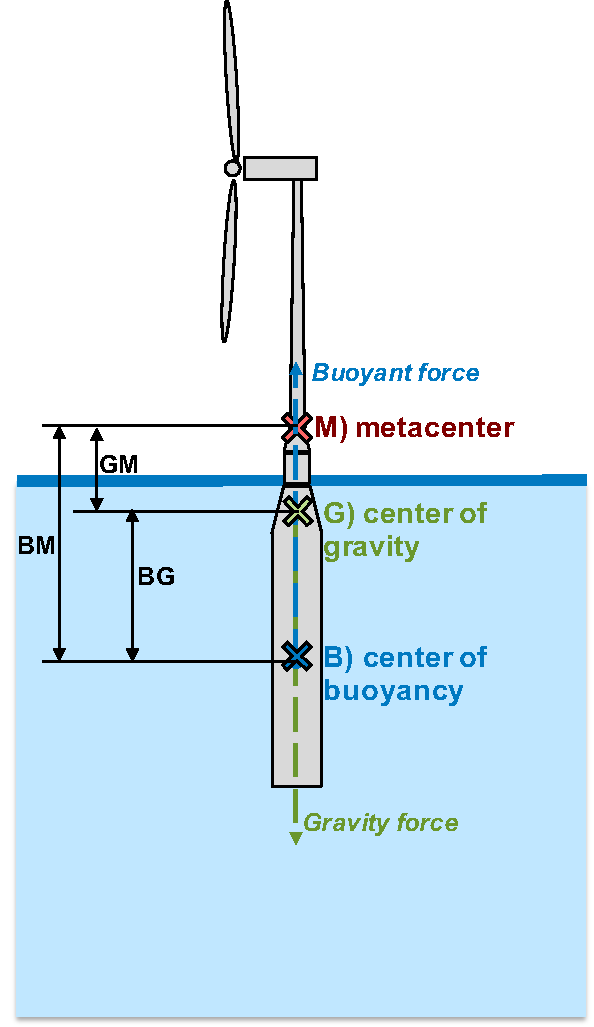
\includegraphics[height=3.5in]{figs/metacenterA.pdf}
    \caption{}
  \end{subfigure}
  \begin{subfigure}[b]{0.49\linewidth}
    \centering 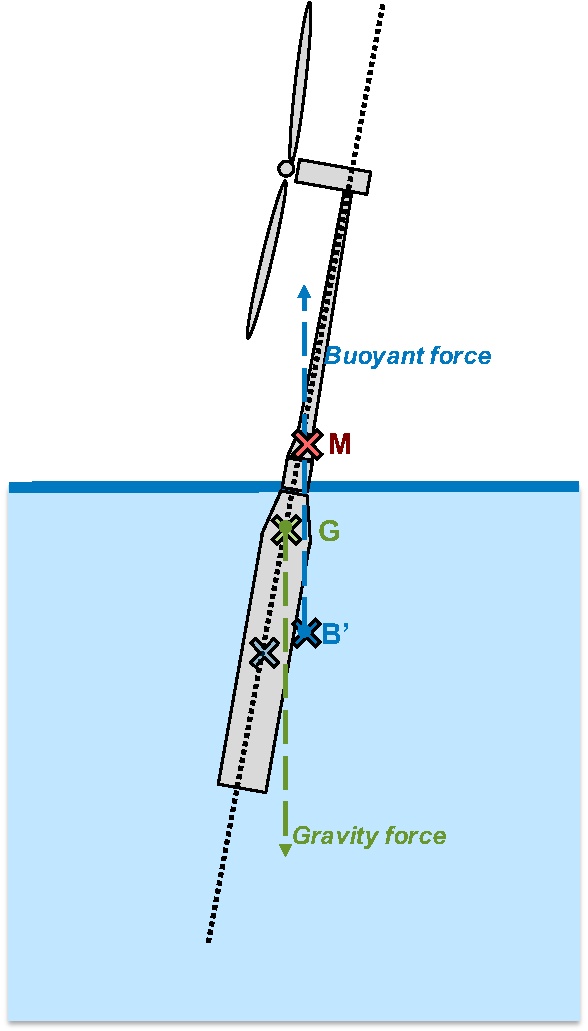
\includegraphics[height=3.5in]{figs/metacenterB.pdf}
    \caption{}
  \end{subfigure}\\
  \caption{Static stability of floating offshore wind turbines.}
  \label{fig:metacenter}
\end{figure}

The second contributing restoring moment comes from the motion of the
center of buoyancy away from alignment with the center of mass.  This is
a standard calculation in naval architecture \citep{thiagarajan2014} and is
diagrammed in Figure \ref{fig:metacenter}.  In this diagram, the center
of mass is denoted, $G$, the center of buoyancy is $B$, and the
metacenter is $M$.  In neural conditions (Figure \ref{fig:metacenter}a),
all of these points are vertically aligned.

As the structure lists or heels, the center of buoyancy shifts toward
the side of the structure that is more submerged (from $B$ to $B'$) and
the buoyancy force no longer passes through the center of mass.
Instead, the buoyancy force passes through the metacenter with an
effective moment arm of $GZ$ from the center of mass (Figure
\ref{fig:metacenter}b).  The metacenter is defined as the common point
through which the buoyancy force acts as it pitches through small
displacements, for bodies with sufficient freeboard margin.

The metacenteric height, $GM$ is most easily calculated as an offset from the
center of buoyancy ($BM$) by,
\[
  h_{meta} = M - G = GM = BM + BG;\quad BM = \frac{I_w}{V}
\]
where $BG$, the distance between the centers of buoyancy and gravity is
easily calculated, $I_w$ is the second moment of area of the substructure waterplane
(with units of \unit{$m^4$}) and $V$ is the total volume of displacement
(with units of \unit{$m^3$}).  Note that for semisubmersible type
geometries, $I_w$ is calculated with the parallel axis theorem for all
of the columns at the waterplane,
\[
  I_w = \sum_i \left( I_{w,i} + S_ir_i^2 \right)
\]
where $S_i$ is the waterplane cross sectional area of the $i$\th column and $r_i$
is the distance from the waterplane centroid to the $i$\th column centroid.

To compute the restoring moment created by the buoyancy force, the first
step is the calculation of the effective moment arm, $GZ$,
\[
GZ = GM \sin \varphi
\]
where $\varphi$ is the angle of heel.  The restoring moment is then the
buoyancy force acting through the restoring arm, $GZ$,
\[
  M_{meta} = F_B \left(GZ\right)
\]
For this reason, the metacenter must be located above the center of mass
for static stability.  This condition is imposed on the design as an
optimization constraint.  Note that the total volume of displacement,
and the subsequent buoyancy force, is not recalculated in the perturbed
configuration.  It is assumed that the angles of deflection are small
and that there is sufficient freeboard and design symmetry such that the
total displacement is constant.

The total restoring pitching moment is then the sum of two
contributions,
\[
  M_{y,restore} = M_{y,moor} + M_{meta}
\]

\section{Hydrostatic Stability}
Floating bodies are typically modeled, for small motions and linearized
behavior, as a second-order differential system with mass, damping, and
spring stiffness terms,
\[
  \left(\mbf{M} + \mbf{A}\right)\ddot{\mbf{x}} + \mbf{C}\dot{\mbf{x}} +
  \mbf{K} = \mbf{F}\left( t \right)
\]
where $\mbf{x}\in\mcal{R}^6$ is the six-degree of freedom vector
(commonly ordered as 1. surge, 2. sway, 3. heave, 4. roll, 5. pitch,
6. yaw), $\mbf{M}$ is the mass matrix, $\mbf{A}$ is the added mass
matrix, $\mbf{C}$ is the damping matrix, and $\mbf{K}$ is the stiffness
matrix.  The right-hand side of the equation captures the time-dependent
summation of all forces.

As a low-fidelity, quasi-static sizing and cost module,
\textit{FloatingSE} does not attempt to capture all of the matrix
entries or forcing terms of the hydrodynamics.  A more sophisticated
time- or frequency-domain solver, where these quantities are calculated, may be linked or included into
\textit{FloatingSE} in the future.  Nevertheless, it does however attempt
to compute the diagonal entries of the mass and stiffness matrices in
order to derive the rigid body natural frequencies of the system,
\[
  \omega_i = \sqrt{\frac{K_{ii}}{M_{ii}+A_{ii}}} \forall i in \left[1\ldots6\right] 
\]
The mass matrix diagonal entries, $M_{ii}$ are simply the mass and
moments of inertia of the whole system,
\[
  M_{11} = M_{22} = M_{33} = m_{sys};\quad M_{44} = I_{xx,sys};\quad M_{55} = I_{yy,sys};\quad M_{66} = I_{zz,sys};
\]
Where the coordinate system notation is consistent with that of Figure
\ref{fig:diagram}.

The added mass matrix diagonal entries are evaluated via standard strip
theory for the tapered columns.  The added mass for the system is a
summation over the columns, using the parallel axis theorem for the
rotational degrees of freedom.  The column quantities are calculated as,
\[
  A_{11} = A_{22} = \rho V;\quad A_{33} = 
  \left(\frac{1}{2}\right)\frac{8}{3} \rho \max R^3(z) ;\quad A_{44} =
  A_{55} = \pi\rho\int\left(z-z_{cb}\right)R^2(z)dz;\quad A_{66} = 0.0;
\]
where $\rho$ is the water density, $R(z)$ is the column radius along its
axis, and $V$ is the submerged volume.  The extra factor of $1/2$ in
$A_{33}$ is included to account for the fact that the top of the column
extends above the waterline.  Also, the integral in $A_{55}$ is only evaluated
along the submerged portion of the column.

The stiffness matrix is comprised of contributions from the mooring
and hydrostatic stiffness.  The mooring linearized stiffness matrix is output
directly from MAP++ and needs no additional processing within
\textit{FloatingSE}.  The hydrostatic stiffness, for a vertical column, is derived from the same
principals described above regarding the metacentric height,
\[
  K_{ii} = K_{ii}^{moor} + K_{ii}^{hydro};\quad K_{33}^{hydro} = \rho g
  S;\quad K_{44}^{hydro} =  K_{55}^{hydro} = \rho g V h_{meta}
\]
where $S$ is the waterplane area of the system.

\chapter{Execution}
\label{sec:exec}
Executing \textit{FloatingSE} requires additional inputs beyond those of
the geometry definition described above in Section \ref{sec:geom}.
Other user inputs for the metocean and loading environment, and the
operational constraints, are required to evaluate the total mass, cost,
and code compliance.  These variables are described below, followed by
the sequence of \textit{FloatingSE} calculations.

\section{User Inputs}
The remaining input variables beyond those listed in Section
\ref{sec:geom} describe the metocean environment, the turbine geometry
and loading, as well as loading constraints.  The loading constraints
are more relevant in the context of optimization, so they are described
later in Section \ref{sec:opt}.  The remaining variables are explained
below.

\subsection{Metocean Environment}
The metocean condition is specified by the water and wind environment.
Geographical dependence is chiefly captured by specifying the water
depth.  The wave loading is parameterized by setting the significant
wave height, periodicity, and mean current speed (if any).  Physical
properties of the water, specifically the density and viscosity, are
also captured.  The user may also set the added mass constant used in
Equation \ref{eqn:morison} (Morison's equation).  All of these variables
cumulatively are in Table \ref{tbl:metocean}

\begin{table}[htbp] \begin{center}
    \caption{Variables specifying the wave environment within \textit{FloatingSE}.}
    \label{tbl:metocean}
{\footnotesize
  \begin{tabular}{ l l c l } \hline
    \textbf{Variable} & \textbf{Type} & \textbf{Units} & \textbf{Description} \\
    \mytt{water\_depth} & Float scalar & $m$& Distance to sea floor \\
    \mytt{hmax}        & Float scalar & $m$& Significant wave height \\
    \mytt{T}           & Float scalar & $s$& Wave period \\
    \mytt{cm}          & Float scalar && Added mass coefficient\\
    \mytt{Uc}          & Float scalar & $m/s$& Mean current speed \\
    \mytt{z0}          & Float scalar & $m$& z-coordinate of water line \\
    \mytt{water\_density}      & Float scalar & $kg/m^3$& Density of water \\
    \mytt{base.waveLoads.mu}  & Float scalar & $kg/m/s$& Viscosity of water \\
  \hline \end{tabular}
}
\end{center} \end{table}

Not that the some of these variables, especially the one setting water
viscosity, are awkwardly named.  This is due
to the need for OpenMDAO to have only one formal independent variable in any
high-level group.  Since \textit{FloatingSE} is intended to be married
with other WISDEM modules in simulation of a full turbine, the design
load cases must be specified at this higher-level group.  Thus,
\textit{FloatingSE} cannot declare independent variables relevant to the
load cases on its own, and must therefore use the variable names as
written in the module code.

The wind profile is specified by the user with a reference height and
velocity.  From there, wind speeds at other heights are determined using
a shear exponent, for power-law scaling, althrough logarithmic scaling
is available as well.  The physical properties of the air at the turbine
location must also be set.  As with the water-relevant variables, the
comment of awkwardly labeled variables applies.  Cumulatively, all of
the wind-related variables are in Table \ref{tbl:windvar}.

\begin{table}[htbp] \begin{center}
    \caption{Variables specifying the wind environment within \textit{FloatingSE}.}
    \label{tbl:windvar}
{\footnotesize
  \begin{tabular}{ l l c l } \hline
    \textbf{Variable} & \textbf{Type} & \textbf{Units} & \textbf{Description} \\
    \mytt{Uref}        & Float scalar & $m/s$& Wind reference speed \\
    \mytt{zref}        & Float scalar & $m$& Wind reference height \\
    \mytt{shearExp}    & Float scalar && Shear exponent in wind power law\\
    \mytt{beta}        & Float scalar & $deg$& Wind beta angle \\
    \mytt{base.windLoads.rho} & Float scalar & $kg/m^3$& Density of air \\
    \mytt{base.windLoads.mu}  & Float scalar & $kg/m/s$& Viscosity of air \\
  \hline \end{tabular}
}
\end{center} \end{table}

As mentioned in Section \ref{sec:theory}, only a single load case is
currently supported.  Future development will allow for optimization
around multiple load cases, each with their own metocean environment.


\subsection{Turbine Description}
To successfully analyze the entire load path through the substructure,
the user, or other WISDEM modules, must input the geometry and loading of
the wind turbine above the substructure.  The next component after the
substructure in the load path is the tower.  As a long, slender column,
the tower geometry parameterization is similar to that of the
substructure columns and has similar variable names, listed in Table
\ref{tbl:towervar}.

\begin{table}[htbp] \begin{center}
    \caption{Variables specifying the tower geometry within \textit{FloatingSE}.}
    \label{tbl:towervar}
{\footnotesize
  \begin{tabular}{ l l c l } \hline
    \textbf{Variable} & \textbf{Type} & \textbf{Units} & \textbf{Description} \\
    \mytt{hub\_height}              & Float scalar & $m$& Length from tower base to top (not including freeboard) \\
    \mytt{tower\_section\_height}    & Float array ($n_s$) & $m$& Length of each tower section \\
    \mytt{tower\_outer\_diameter}    & Float array ($n_s+1$) & $m$& Diameter at each tower section node (linear lofting between) \\
    \mytt{tower\_wall\_thickness}    & Float array ($n_s+1$) & $m$& Diameter at each tower section node (linear lofting between) \\
    \mytt{tower\_buckling\_length}   & Float scalar & $m$& Tower buckling reinforcement spacing \\
    \mytt{tower\_outfitting\_factor} & Float scalar && Scaling for unaccounted tower mass in outfitting\\
  \hline \end{tabular}
}
\end{center} \end{table}


At the top of the load path, above the tower, is the rotor nacelle
assembly (RNA).  The RNA includes the blades, hub, shaft(s), gearbox,
generator, nacelle housing, etc.  All of these components are addressed
separately across multiple WISDEM modules, but \textit{FloatingSE} only
requires aggregate summations of the mass properties, forces, and
moments.  These cumulative variables are in Table \ref{tbl:rnavar}.

\begin{table}[htbp] \begin{center}
    \caption{Variables specifying the RNA geometry and loads within \textit{FloatingSE}.}
    \label{tbl:rnavar}
{\footnotesize
  \begin{tabular}{ l l c l } \hline
    \textbf{Variable} & \textbf{Type} & \textbf{Units} & \textbf{Description} \\
    \mytt{rna\_mass}   & Float scalar & $kg$& Mass \\
    \mytt{rna\_I}      & Float array (6) & $kg/m^2$& Moment of intertia (xx,yy,zz,xy,xz,yz) \\
    \mytt{rna\_cg}     & Float array (3) & $m$& Offset of RNA center of mass from tower top (x,y,z) \\
    \mytt{rna\_force}  & Float array (3) & $N$& Net force acting on RNA (x,y,z) \\
    \mytt{rna\_moment} & Float array (3) & $N*m$& Net moment acting on RNA (x,y,z) \\
    \mytt{yaw}         & Float scalar && Turbine yaw angle\\
  \hline \end{tabular}
}
\end{center} \end{table}


\section{Simulation Flow}
Once the input variables are completely specified, \textit{FloatingSE}
executes the analysis of the substructure.  Conceptually, the simulation
is organized by the flowchart in Figure \ref{fig:floatingse}.  From a
more technical perspective, \textit{FloatingSE} is an OpenMDAO Group, so
the analysis sequence is broken down by the sub-groups and
sub-components in the order that they are listed in Table
\ref{tbl:exec}.  In an OpenMDAO group, sub-groups and components are
given prefixes to aid in referring to specific variables.  The prefixes
used in \textit{FloatingSE} are also listed in Table \ref{tbl:exec}.
These prefixes also appear in some of the variable names listed above (e.g.,
\texttt{base.waveLoads.mu}) and will appear in the discussion of
optimization constraints in Section \ref{sec:opt}.

\begin{table}[htbp] \begin{center}
    \caption{Components and sub-groups within \textit{FloatingSE}.}
    \label{tbl:exec}
{\small
  \begin{tabular}{ l l l l } \hline
    &  \textbf{Prefix} & \textbf{Name} & \textbf{Description} \\ \hline\hline
    1) & \texttt{tow} & \textit{TowerLeanSE} & Discretization of tower
    geometry (but no analysis) \\
    2) & \texttt{base} & \textit{Column} & Discretization and API
    Bulletin 2U compliance of base vertical column \\
    3) & \texttt{aux} & \textit{Column} & Discretization and API
    Bulletin 2U compliance of auxiliary columns \\
    4) & \texttt{load} & \textit{FloatingLoading} & Structural analysis
    of comoplete floating turbine load path using \textit{pyFrame3DD} \\
    5) & \texttt{sg} & \textit{SubstructureGeometry} & Geometrical constraints
    on substructure \\
    6) & \texttt{mm} & \textit{MapMooring} & Mooring system analysis using MAP++ program \\
    7) & \texttt{stab} & \textit{SemiStable} & Static stability and final mass and cost summation for generic substructure \\
  \hline \end{tabular}
}
\end{center} \end{table}

\begin{figure}[htb]
  \begin{center}
    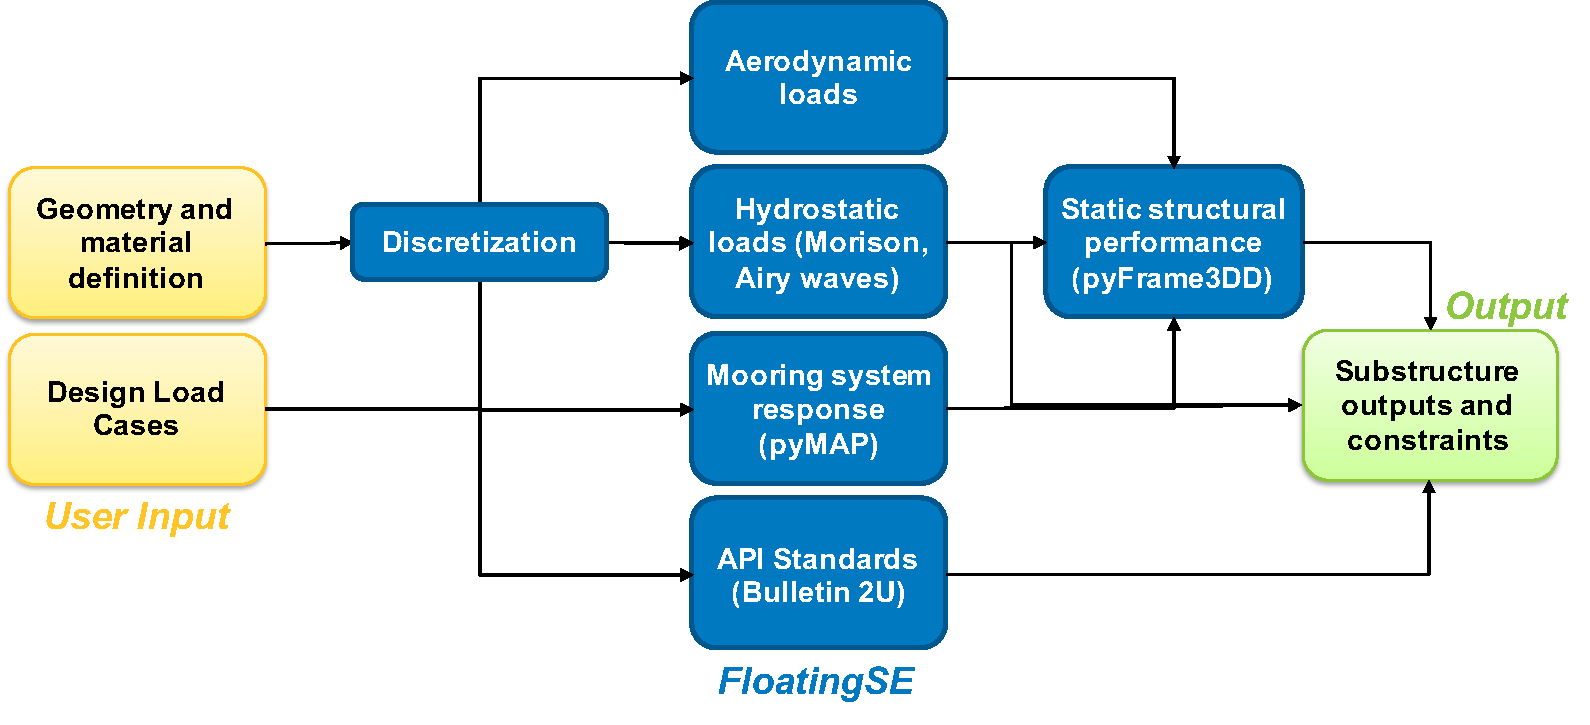
\includegraphics[width=5in]{figs/floatingse.pdf}
    \caption{Conceptual diagram of \textit{FloatingSE} execution.}
    \label{fig:floatingse}
  \end{center}
\end{figure}

Outputs are accumulated in each sub-group or component,
and they either become inputs to other components, become constraints
for optimization problems, become design variables for optimization
problems, or can simply be ignored.  Currently, a single execution of
FloatingSE takes only a handful of seconds on a modern laptop computer.


\section{Examples}
As mentioned in Section \ref{sec:package}, two files are meant as
analysis starting points, \texttt{sparInstance.py} and
\texttt{semiInstance.py}.  These files are encoded with default starting
configurations (from \citet{OC3} and \citet{OC4}, respectively).  They
also have ready configurations for optimization with design variables,
constraints, and solvers options.  However, due to the flexible and
object-oriented approach to programming these capabilities, some
complexity was introduced into the code and it is difficult to use as
simple examples.  For demonstration purposes, the spar and
semisubmersible examples from OC3 and OC4 are also provided at the
bottom of the \texttt{floating.py} file, and are copied below.  A
visualization of the geometries described by these examples is shown in
Figure \ref{fig:initial}

\begin{figure}[htb]
  \begin{subfigure}[b]{0.49\linewidth}
    \centering 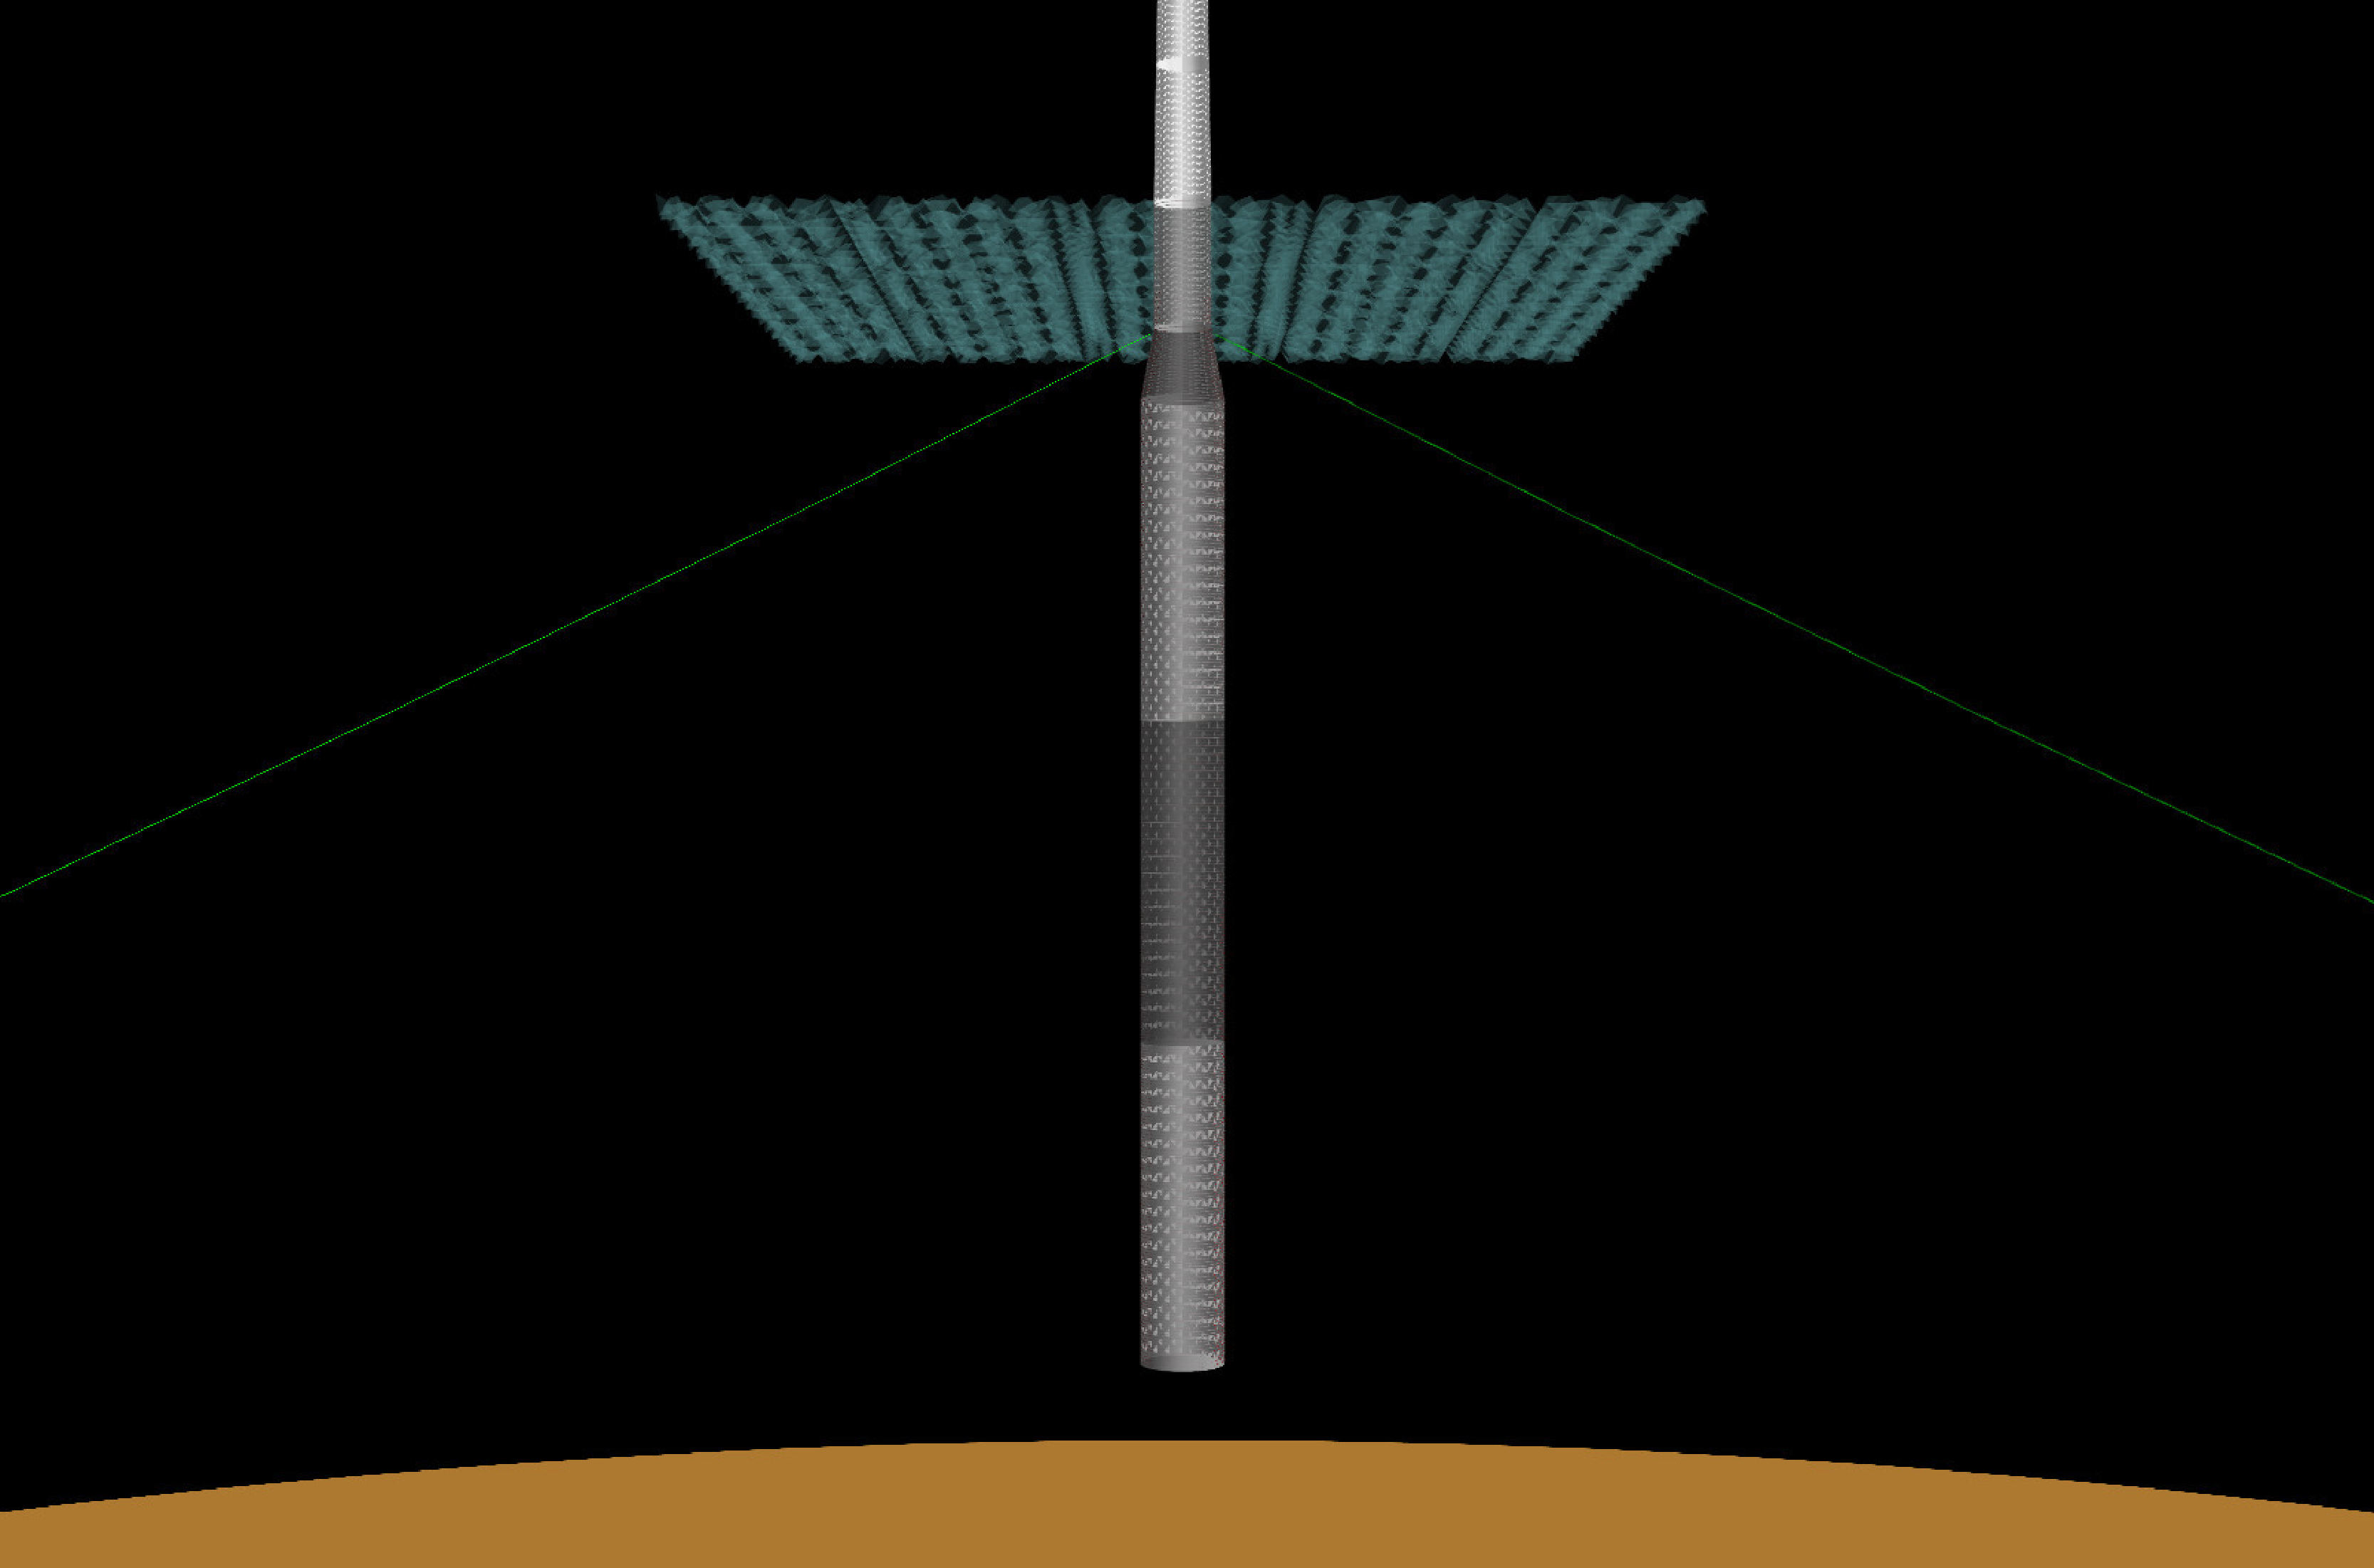
\includegraphics[width=\linewidth]{figs/spar-initial.pdf}
    \caption{Spar}
  \end{subfigure}
  \begin{subfigure}[b]{0.49\linewidth}
    \centering 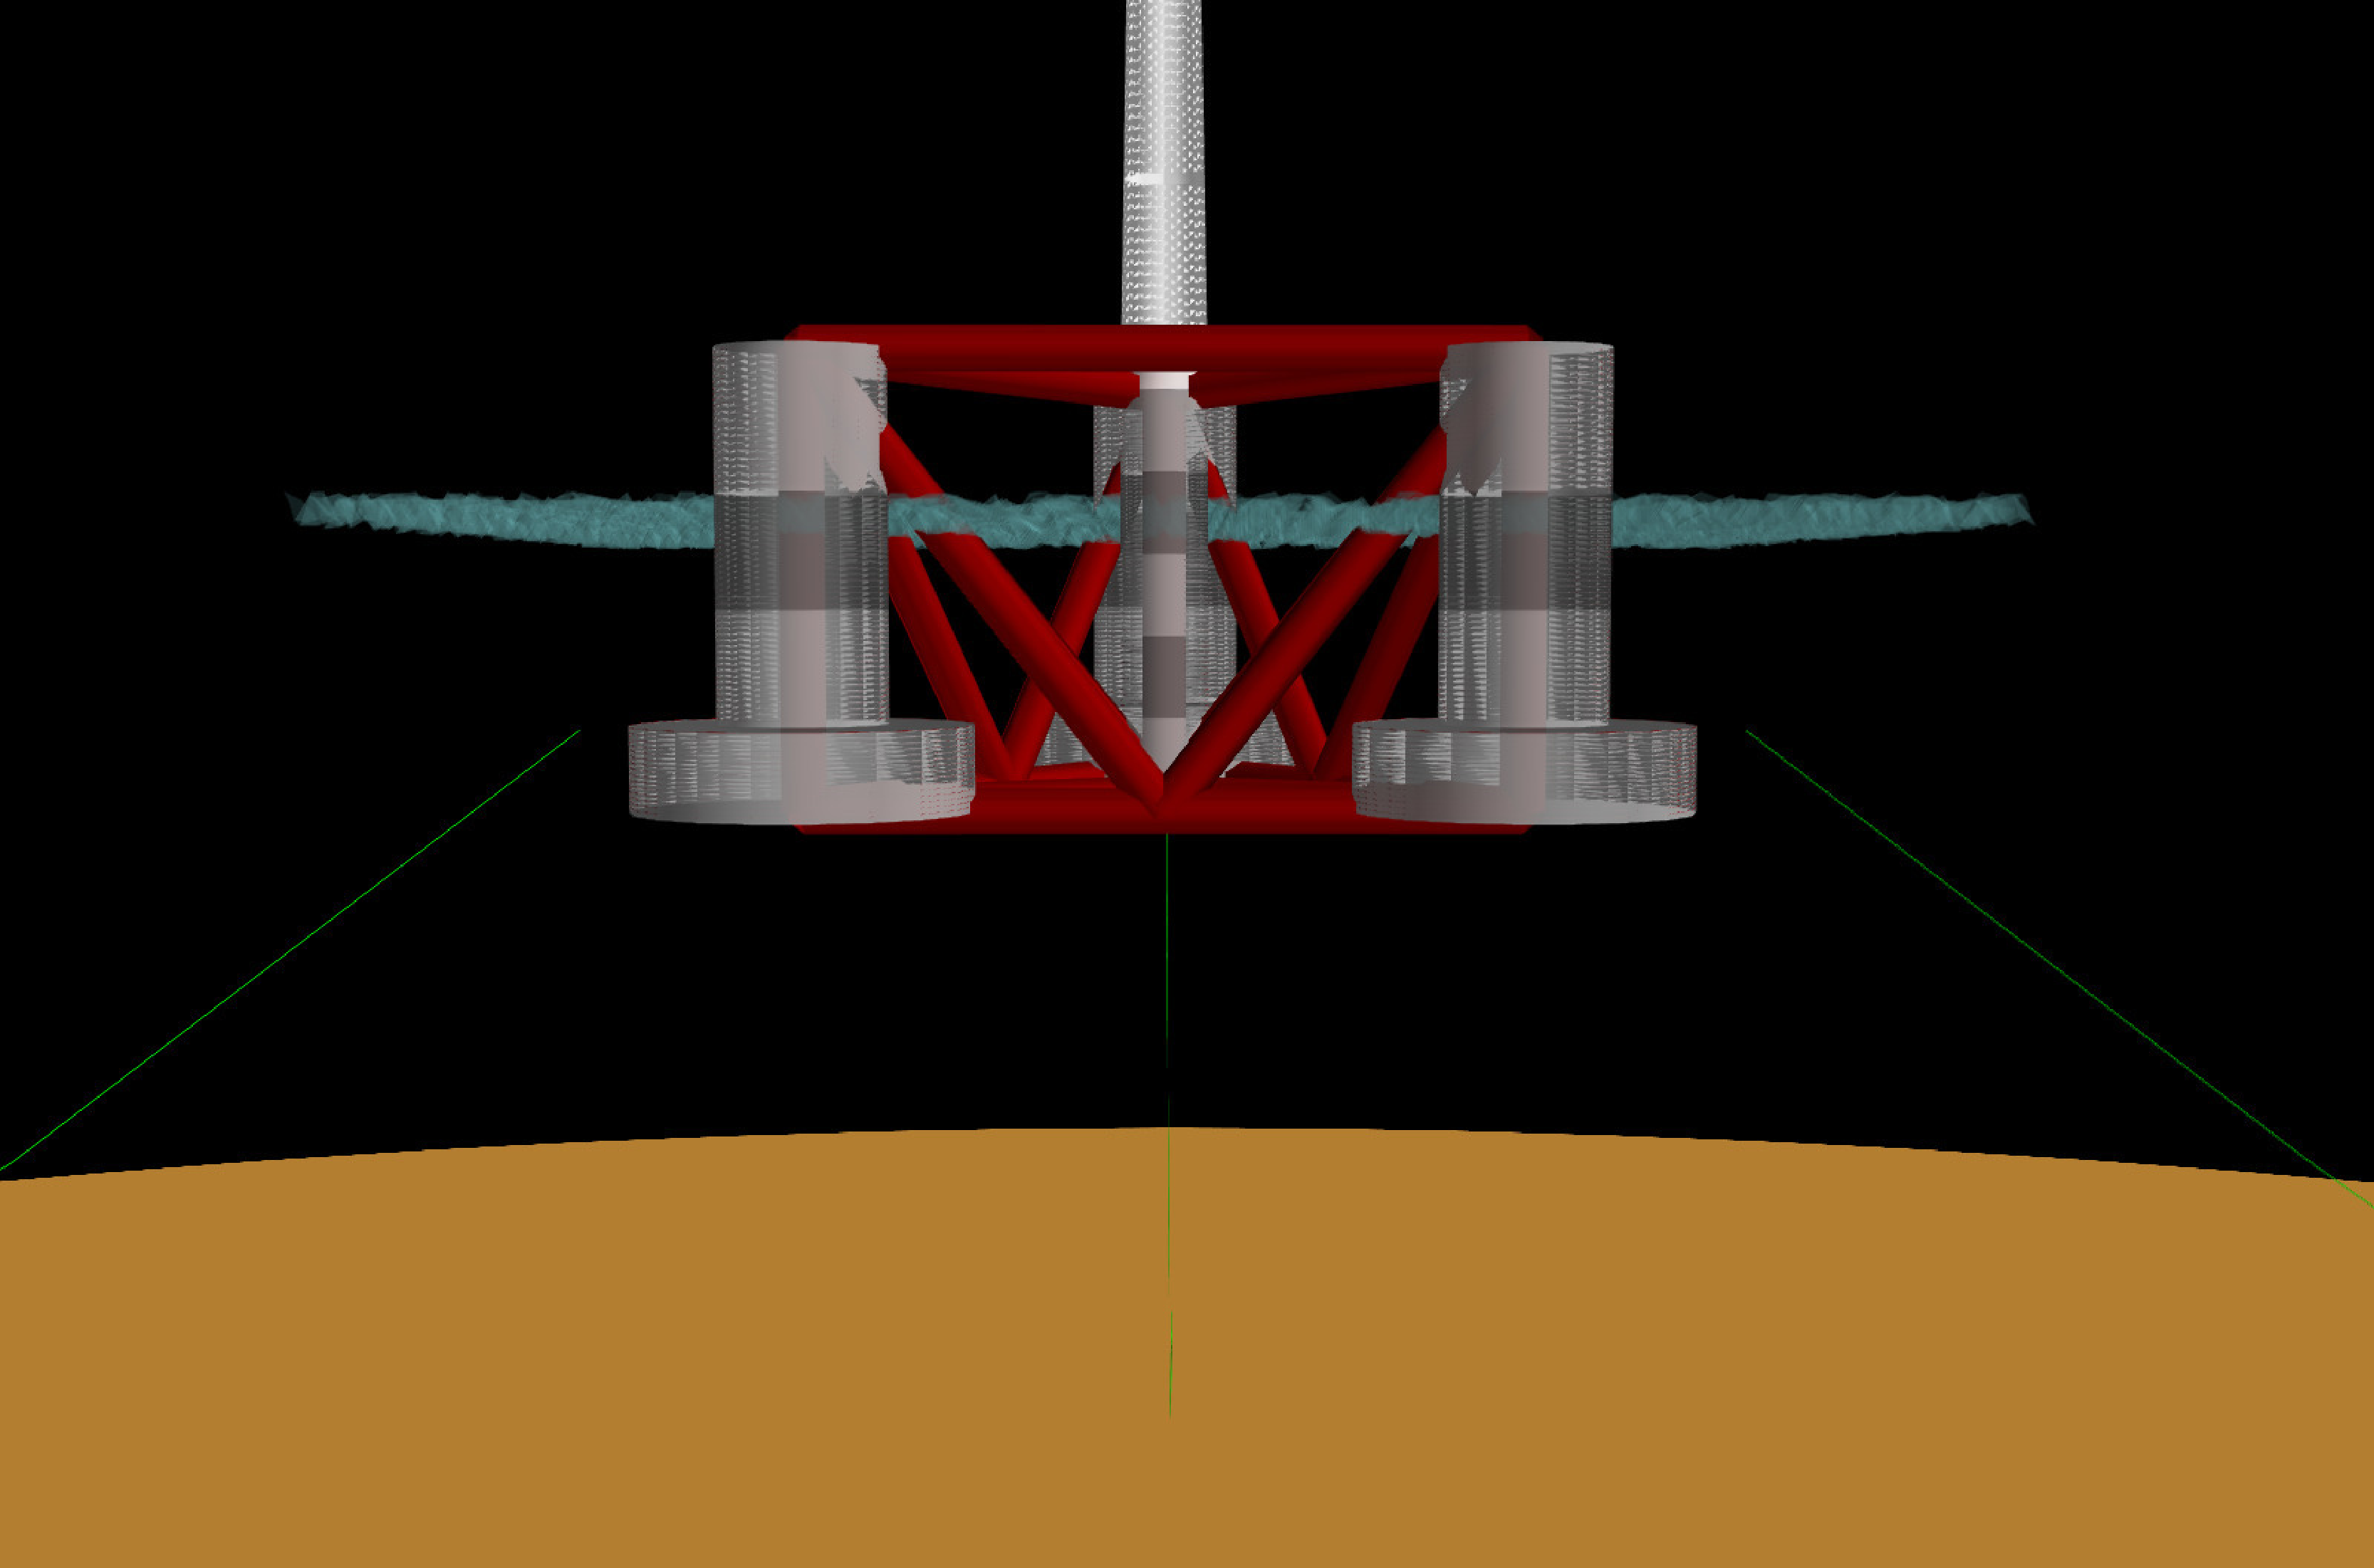
\includegraphics[width=\linewidth]{figs/semi-initial.pdf}
    \caption{Semisubmersible}
  \end{subfigure}\\
  \caption{Spar and semisubmersible examples in \textit{FloatingSE} taken from
    OC3\citep{OC3} and OC4\citep{OC4} projects.}
  \label{fig:initial}
\end{figure}

\subsection{Spar and Semisubmersible}

\begin{lstlisting}
# Wind and water properties
prob['base.windLoads.rho'] = 1.226   # Density of air [kg/m^3]
prob['base.windLoads.mu']  = 1.78e-5 # Viscosity of air [kg/m/s]
prob['water_density']      = 1025.0  # Density of water [kg/m^3]
prob['base.waveLoads.mu']  = 1.08e-3 # Viscosity of water [kg/m/s]

# Material properties
prob['material_density'] = 7850.0          # Steel [kg/m^3]
prob['E']                = 200e9           # Young's modulus [N/m^2]
prob['G']                = 79.3e9          # Shear modulus [N/m^2]
prob['yield_stress']     = 3.45e8          # Elastic yield stress [N/m^2]
prob['nu']               = 0.26            # Poisson's ratio
prob['permanent_ballast_density'] = 4492.0 # [kg/m^3]

# Mass and cost scaling factors
prob['bulkhead_mass_factor']     = 1.0     # Scaling for unaccounted bulkhead mass
prob['ring_mass_factor']         = 1.0     # Scaling for unaccounted stiffener mass
prob['shell_mass_factor']        = 1.0     # Scaling for unaccounted shell mass
prob['column_mass_factor']       = 1.05    # Scaling for unaccounted column mass
prob['outfitting_mass_fraction'] = 0.06    # Fraction of additional outfitting mass for each column
prob['ballast_cost_rate']        = 100.0   # Cost factor for ballast mass [USD/kg]
prob['tapered_col_cost_rate']    = 4720.0  # Cost factor for column mass [USD/kg]
prob['outfitting_cost_rate']     = 6980.0  # Cost factor for outfitting mass [USD/kg]
prob['mooring_cost_rate']        = 1.1     # Cost factor for mooring mass [USD/kg]

# Safety factors
prob['gamma_f'] = 1.35 # Safety factor on loads
prob['gamma_b'] = 1.1  # Safety factor on buckling
prob['gamma_m'] = 1.1  # Safety factor on materials
prob['gamma_n'] = 1.0  # Safety factor on consequence of failure
prob['gamma_fatigue'] = 1.755 # Not used

# Porperties of turbine tower
prob['hub_height']              = 77.6                              # Length from tower base to top (not including freeboard) [m]
prob['tower_section_height']    = 77.6/nsection * np.ones(nsection) # Length of each tower section [m]
prob['tower_outer_diameter']    = np.linspace(6.5, 3.87, nsection+1) # Diameter at each tower section node (linear lofting between) [m]
prob['tower_wall_thickness']    = np.linspace(0.027, 0.019, nsection+1) # Diameter at each tower section node (linear lofting between) [m]
prob['tower_buckling_length']   = 30.0                              # Tower buckling reinforcement spacing [m]
prob['tower_outfitting_factor'] = 1.07                              # Scaling for unaccounted tower mass in outfitting

# Properties of rotor-nacelle-assembly (RNA)
prob['rna_mass']   = 350e3 # Mass [kg]
prob['rna_I']      = 1e5*np.array([1149.307, 220.354, 187.597, 0, 5.037, 0]) # Moment of intertia (xx,yy,zz,xy,xz,yz) [kg/m^2]
prob['rna_cg']     = np.array([-1.132, 0, 0.509])                       # Offset of RNA center of mass from tower top (x,y,z) [m]
# Max thrust
prob['rna_force']  = np.array([1284744.196, 0, -112400.5527])           # Net force acting on RNA (x,y,z) [N]
prob['rna_moment'] = np.array([3963732.762, 896380.8464, -346781.682]) # Net moment acting on RNA (x,y,z) [N*m]
# Max wind speed
#prob['rna_force']  = np.array([188038.8045, 0,  -16451.2637]) # Net force acting on RNA (x,y,z) [N]
#prob['rna_moment'] = np.array([0.0, 131196.8431,  0.0]) # Net moment acting on RNA (x,y,z) [N*m]
\end{lstlisting}

\subsection{Spar Only}
The common declarations above should be inserted in the midst of the
variable declarations below.

\begin{lstlisting}
# Number of sections to be used in the design
nsection = 5

# Initialize OpenMDAO problem and FloatingSE Group
prob = Problem(root=FloatingSE(nsection))
prob.setup()

# Remove all auxiliary columns
prob['number_of_auxiliary_columns'] = 0
prob['cross_attachment_pontoons']   = False
prob['lower_attachment_pontoons']   = False
prob['upper_attachment_pontoons']   = False
prob['lower_ring_pontoons']         = False
prob['upper_ring_pontoons']         = False
prob['outer_cross_pontoons']        = False

# Set environment to that used in OC3 testing campaign
prob['water_depth'] = 320.0  # Distance to sea floor [m]
prob['hmax']        = 10.8   # Significant wave height [m]
prob['T']           = 9.8    # Wave period [s]
prob['Uref']        = 11.0   # Wind reference speed [m/s]
prob['zref']        = 119.0  # Wind reference height [m]
prob['shearExp']    = 0.11   # Shear exponent in wind power law
prob['cm']          = 2.0    # Added mass coefficient
prob['Uc']          = 0.0    # Mean current speed
prob['z0']          = 0.0    # Water line
prob['yaw']         = 0.0    # Turbine yaw angle
prob['beta']        = 0.0    # Wind beta angle
prob['cd_usr']      = np.inf # Compute drag coefficient

# Column geometry
prob['base_permanent_ballast_height'] = 10.0 # Height above keel for permanent ballast [m]
prob['base_freeboard']                = 10.0 # Height extension above waterline [m]
prob['base_section_height'] = np.array([36.0, 36.0, 36.0, 8.0, 14.0])  # Length of each section [m]
prob['base_outer_diameter'] = np.array([9.4, 9.4, 9.4, 9.4, 6.5, 6.5]) # Diameter at each section node (linear lofting between) [m]
prob['base_wall_thickness'] = 0.05 * np.ones(nsection+1)               # Shell thickness at each section node (linear lofting between) [m]
prob['base_bulkhead_nodes'] = [True, True, False, False, False, False] # Locations of internal bulkheads at section interfaces

# Column ring stiffener parameters
prob['base_stiffener_web_height']       = 0.10 * np.ones(nsection) # (by section) [m]
prob['base_stiffener_web_thickness']    = 0.04 * np.ones(nsection) # (by section) [m]
prob['base_stiffener_flange_width']     = 0.10 * np.ones(nsection) # (by section) [m]
prob['base_stiffener_flange_thickness'] = 0.02 * np.ones(nsection) # (by section) [m]
prob['base_stiffener_spacing']          = 0.40 * np.ones(nsection) # (by section) [m]

# Mooring parameters
prob['number_of_mooring_lines']    = 3             # Evenly spaced around structure
prob['mooring_type']               = 'chain'       # Options are chain, nylon, polyester, fiber, or iwrc
prob['anchor_type']                = 'suctionpile' # Options are SUCTIONPILE or DRAGEMBEDMENT
prob['mooring_diameter']           = 0.09          # Diameter of mooring line/chain [m]
prob['fairlead']                   = 70.0          # Distance below waterline for attachment [m]
prob['fairlead_offset_from_shell'] = 0.5           # Offset from shell surface for mooring attachment [m]
prob['scope_ratio']                = 3.6088        # Ratio of line length to distance to sea floor (from fairlead)
prob['anchor_radius']              = 853.87        # Distance from centerline to sea floor landing [m]
prob['drag_embedment_extra_length'] = 300.0        # Extra length beyond sea flor landing to ensure anchors only see horizontal forces [m]

# Execute FloatingSE
prob.run()

\end{lstlisting}

\subsection{Semisubmersible Only}
The common declarations above should be inserted in the midst of the
variable declarations below.
\begin{lstlisting}
# Number of sections to be used in the design
nsection = 5

# Initialize OpenMDAO problem and FloatingSE Group
prob = Problem(root=FloatingSE(nsection))
prob.setup()

# Add in auxiliary columns and truss elements
prob['number_of_auxiliary_columns'] = 3
prob['cross_attachment_pontoons']   = True # Lower-Upper base-to-auxiliary connecting cross braces
prob['lower_attachment_pontoons']   = True # Lower base-to-auxiliary connecting pontoons
prob['upper_attachment_pontoons']   = True # Upper base-to-auxiliary connecting pontoons
prob['lower_ring_pontoons']         = True # Lower ring of pontoons connecting auxiliary columns
prob['upper_ring_pontoons']         = True # Upper ring of pontoons connecting auxiliary columns
prob['outer_cross_pontoons']        = True # Auxiliary ring connecting V-cross braces

# Set environment to that used in OC4 testing campaign
prob['water_depth'] = 200.0  # Distance to sea floor [m]
prob['hmax']        = 10.8   # Significant wave height [m]
prob['T']           = 9.8    # Wave period [s]
prob['Uref']        = 11.0   # Wind reference speed [m/s]
prob['zref']        = 119.0  # Wind reference height [m]
prob['shearExp']    = 0.11   # Shear exponent in wind power law
prob['cm']          = 2.0    # Added mass coefficient
prob['Uc']          = 0.0    # Mean current speed
prob['z0']          = 0.0    # Water line
prob['yaw']         = 0.0    # Turbine yaw angle
prob['beta']        = 0.0    # Wind beta angle
prob['cd_usr']      = np.inf # Compute drag coefficient

# Column geometry
prob['base_permanent_ballast_height'] = 10.0 # Height above keel for permanent ballast [m]
prob['base_freeboard']                = 10.0 # Height extension above waterline [m]
prob['base_section_height'] = np.array([36.0, 36.0, 36.0, 8.0, 14.0])  # Length of each section [m]
prob['base_outer_diameter'] = np.array([9.4, 9.4, 9.4, 9.4, 6.5, 6.5]) # Diameter at each section node (linear lofting between) [m]
prob['base_wall_thickness'] = 0.05 * np.ones(nsection+1)               # Shell thickness at each section node (linear lofting between) [m]
prob['base_bulkhead_nodes'] = [True, True, False, False, False, False] # Locations of internal bulkheads at section interfaces

# Auxiliary column geometry
prob['radius_to_auxiliary_column']         = 33.333 * np.cos(np.pi/6) # Centerline of base column to centerline of auxiliary column [m]
prob['auxiliary_permanent_ballast_height'] = 0.1                      # Height above keel for permanent ballast [m]
prob['auxiliary_freeboard']                = 12.0                     # Height extension above waterline [m]
prob['auxiliary_section_height']           = np.array([6.0, 0.1, 7.9, 8.0, 10]) # Length of each section [m]
prob['auxiliary_outer_diameter']           = np.array([24, 24, 12, 12, 12, 12]) # Diameter at each section node (linear lofting between) [m]
prob['auxiliary_wall_thickness']           = 0.06 * np.ones(nsection+1)         # Shell thickness at each section node (linear lofting between) [m]

# Column ring stiffener parameters
prob['base_stiffener_web_height']       = 0.10 * np.ones(nsection) # (by section) [m]
prob['base_stiffener_web_thickness']    = 0.04 * np.ones(nsection) # (by section) [m]
prob['base_stiffener_flange_width']     = 0.10 * np.ones(nsection) # (by section) [m]
prob['base_stiffener_flange_thickness'] = 0.02 * np.ones(nsection) # (by section) [m]
prob['base_stiffener_spacing']          = 0.40 * np.ones(nsection) # (by section) [m]

# Auxiliary column ring stiffener parameters
prob['auxiliary_stiffener_web_height']       = 0.10 * np.ones(nsection) # (by section) [m]
prob['auxiliary_stiffener_web_thickness']    = 0.04 * np.ones(nsection) # (by section) [m]
prob['auxiliary_stiffener_flange_width']     = 0.01 * np.ones(nsection) # (by section) [m]
prob['auxiliary_stiffener_flange_thickness'] = 0.02 * np.ones(nsection) # (by section) [m]
prob['auxiliary_stiffener_spacing']          = 0.40 * np.ones(nsection) # (by section) [m]

# Pontoon parameters
prob['pontoon_outer_diameter']    = 3.2    # Diameter of all pontoon/truss elements [m]
prob['pontoon_wall_thickness']    = 0.0175 # Thickness of all pontoon/truss elements [m]
prob['base_pontoon_attach_lower'] = -20.0  # Lower z-coordinate on base where truss attaches [m]
prob['base_pontoon_attach_upper'] = 10.0   # Upper z-coordinate on base where truss attaches [m]

# Mooring parameters
prob['number_of_mooring_lines']    = 3             # Evenly spaced around structure
prob['mooring_type']               = 'chain'       # Options are chain, nylon, polyester, fiber, or iwrc
prob['anchor_type']                = 'suctionpile' # Options are SUCTIONPILE or DRAGEMBEDMENT
prob['mooring_diameter']           = 0.0766        # Diameter of mooring line/chain [m]
prob['fairlead']                   = 14.0          # Distance below waterline for attachment [m]
prob['fairlead_offset_from_shell'] = 0.5           # Offset from shell surface for mooring attachment [m]
prob['scope_ratio']                = 4.4919        # Ratio of line length to distance to sea floor (from fairlead)
prob['anchor_radius']              = 837.6         # Distance from centerline to sea floor landing [m]
prob['drag_embedment_extra_length'] = 300.0        # Extra length beyond sea flor landing to ensure anchors only see horizontal forces [m]

# Execute FloatingSE
prob.run()
\end{lstlisting}

\chapter{Optimization}
\label{sec:opt}
Executing \textit{FloatingSE} by hand is sufficient to explore some simple
one-off or comparison analyses between a few runs.  OpenMDAO
provides extensive optimization capability, which can give yield richer
and more insightful analyses.  Beyond setting initial conditions for all
of the input variables, the user must also specify,
\begin{description}
\item[Design Variables]: The variables that are adjusted in order to
  find the optimal solution;
\item[Constraints]: The set of conditions that the solution must satisfy;
\item[Objective(s)]: The metrics used to minimize (or maximize) in the
  optimization problem; 
\item[Solver/Driver]: The algorithm used to find the optimal set of
  design variable values.
\end{description}

\section{Design Variables}
OpenMDAO currently only supports continuous design variables, those that
can take on any decimal value, because gradients with respect to the
objective function can be obtained.  Mixed-integer optimization drivers,
which can handle variables that take on discrete values (e.g. number of
mooring lines, or type of mooring line) are not yet fully implemented.
To realize the full analysis capabilities of \textit{FloatingSE}, an
mixed-integer optimization driver will have to be used.  Thus,
experimenting with this type of approach is in the near-term development
plan.

Aside from the restriction to continuous design variables, the user
could denote any variable as a design variable.  This is in fact a
feature of OpenMDAO, where any variable can be a design
variable, and any output could be a constraint or objective function.
The standard list of design variables in \textit{FloatingSE} given in
the examples are the continuous variables that parametrically describe
the geometry of the substructure listed in Section \ref{sec:geom}.  For
a succinct, central listing, these variables are collected together in
Table \ref{tbl:designvar}.

\begin{table}[htbp] \begin{center}
    \caption{Standard design variables used for optimization in \textit{FloatingSE}.}
    \label{tbl:designvar}
{\footnotesize
  \begin{tabularx}{\textwidth}{ l l c c X } \hline
    \textbf{Variable} & \textbf{Type} & \textbf{Units} & \textbf{Bounds} &\textbf{Description} \\ \hline \hline
    \mytt{base\_section\_height} & Float array ($n_s$) & $m$& 0.1--100&Height of each section \\
    \mytt{base\_outer\_diameter} & Float array ($n_s+1$) & $m$& 1.1--40&Diameter at each section node (linear lofting between)\\
    \mytt{base\_wall\_thickness} & Float array ($n_s+1$)  & $m$& 0.005--1&Wall thickness at each section node (linear lofting between) \\
    \mytt{base\_freeboard} & Float scalar & $m$&0--50 &Design height above waterline\\
    \mytt{base\_stiffener\_web\_height} & Float array ($n_s$) & $m$& 0.01--1&Stiffener web height for each section \\
    \mytt{base\_stiffener\_web\_thickness} & Float array ($n_s$) & $m$& 0.001--0.5&Stiffener web thickness for each section \\
    \mytt{base\_stiffener\_flange\_width} & Float array ($n_s$) & $m$& 0.01--5&Stiffener flange width for each section \\
    \mytt{base\_stiffener\_flange\_thickness} & Float array ($n_s$) & $m$& 0.001--0.5&Stiffener flange thickness for each section\\
    \mytt{base\_stiffener\_spacing} & Float array ($n_s$) & $m$& 0.01--10&Stiffener spacing for each section \\
    \mytt{auxiliary\_section\_height} & Float array ($n_s$) & $m$& 0.1--100&Height of each section \\
    \mytt{auxiliary\_outer\_diameter} & Float array ($n_s+1$)&$m$& 1.1--40&Diameter at each section node (linear lofting between)\\
    \mytt{auxiliary\_wall\_thickness} &Float array ($n_s+1$) &$m$& 0.005--1&Wall thickness at each section node (linear lofting between)\\
    \mytt{auxiliary\_freeboard} & Float scalar & $m$& 0--50 &Design height above waterline \\
    \mytt{auxiliary\_stiffener\_web\_height} & Float array ($n_s$) & $m$& 0.01--1&Stiffener web height for each section \\
    \mytt{auxiliary\_stiffener\_web\_thickness} & Float array ($n_s$) &$m$& 0.001--0.5&Stiffener web thickness for each section\\
    \mytt{auxiliary\_stiffener\_flange\_width} & Float array ($n_s$) &$m$& 0.01--5&Stiffener flange width for each section\\
    \mytt{auxiliary\_stiffener\_flange\_thickness} & Float array ($n_s$) &$m$& 0.001--0.5&Stiffener flange thickness for each section\\
    \mytt{auxiliary\_stiffener\_spacing} & Float array ($n_s$) & $m$& 0.01--10&SStiffener spacing for each section \\
    \mytt{radius\_to\_auxiliary\_column} & Float scalar &$m$& 0--40&Centerline of base column to centerline of auxiliary column\\
    \mytt{base\_permanent\_ballast\_height} & Float scalar & $m$& 0.1--50&Height above keel for permanent ballast \\
    \mytt{auxiliary\_permanent\_ballast\_height} & Float scalar & $m$& 0.1--50&Height above keel for permanent ballast \\
    \mytt{pontoon\_outer\_diameter} & Float scalar & $m$& 0.1--3&Diameter of all pontoon/truss elements \\
    \mytt{pontoon\_wall\_thickness} & Float scalar & $m$& 0.005--0.1&Thickness of all pontoon/truss elements \\
    \mytt{base\_pontoon\_attach\_lower} & Float scalar & $m$& -100--100&Lower z-coordinate on base where truss attaches \\
    \mytt{base\_pontoon\_attach\_upper} & Float scalar & $m$& -100--100&Upper z-coordinate on base where truss attaches \\
    \mytt{mooring\_diameter} & Float scalar & $m$& 0.05--1&Diameter of mooring line/chain \\
    \mytt{fairlead} & Float scalar & $m$& 0--200&Distance below waterline for attachment \\
    \mytt{fairlead\_offset\_from\_shell} & Float scalar & $m$ & 0--5& Offset from shell surface for mooring attachment \\
    \mytt{scope\_ratio} & Float scalar && 1--5&Ratio of line length to distance to sea floor (from fairlead)\\
    \mytt{anchor\_radius} & Float scalar & $m$& 1--1000&Distance from centerline to sea floor landing \\
  \hline \end{tabularx}
}
\end{center} \end{table}


\section{Constraints}
Due to the many design variables, permutations of settings, and applied
physics, there are many constraints that must be applied for an
optimization to close.  These constraints can be tuned with user inputs
and/or user-defined limits for the constraints in the optimization
problem set-up.  The constraints are described in detail in the
following sub-sections.  For convenience, all of the constraints, and
their bounds, are also collected together in Table \ref{tbl:constraints}.

\begin{table}[htbp] \begin{center}
    \caption{Optimization constraints used in \textit{FloatingSE}.}
    \label{tbl:constraints}
    {\footnotesize
  \begin{tabular}{ r l l |c| r l l} \hline
    \textbf{Lower} & \textbf{Constraint} & \textbf{Upper} && \textbf{Lower} & \textbf{Constraint} & \textbf{Upper} \\ \hline \hline
& \mytt{base.draft\_depth\_ratio} & $0.75$ && $1.0$ & \mytt{base.flange\_compactness} &\\
& \mytt{aux.draft\_depth\_ratio} & $0.75$&& $1.0$ & \mytt{base.web\_compactness} &\\
& \mytt{aux.fairlead\_draft\_ratio} & $1.0$&& $1.0$ & \mytt{aux.flange\_compactness} &\\
& \mytt{so.base\_auxiliary\_spacing} & $1.0$&& $1.0$ & \mytt{aux.web\_compactness} &\\
$\unit[0.0]{m}$ & \mytt{sg.transition\_buffer} & $\unit[2.0]{m}$&& & \mytt{base.axial\_local\_unity} & $1.0$\\
& \mytt{base.flange\_spacing\_ratio} & $1.0$&& & \mytt{base.axial\_general\_unity} & $1.0$\\ 
& \mytt{base.web\_radius\_ratio} & $1.0$&& & \mytt{base.external\_local\_unity} & $1.0$\\
& \mytt{aux.flange\_spacing\_ratio} & $1.0$&& & \mytt{base.external\_general\_unity} & $1.0$\\
& \mytt{aux.web\_radius\_ratio} & $1.0$&& & \mytt{aux.axial\_local\_unity} & $1.0$\\
$0.0$ & \mytt{load.pontoon\_base\_attach\_lower} & $0.5$&& & \mytt{aux.axial\_general\_unity} & $1.0$\\
$0.5$ & \mytt{load.pontoon\_base\_attach\_upper} & $1.0$&& & \mytt{aux.external\_local\_unity} & $1.0$\\
$1.0$ & \mytt{mm.mooring\_length\_min} &&& & \mytt{aux.external\_general\_unity} & $1.0$\\ 
& \mytt{mm.mooring\_length\_max} & $1.0$&& & \mytt{load.pontoon\_stress} & $1.0$\\
& \mytt{base.manufacturability} & $0.0$&& & \mytt{load.tower\_stress} & $1.0$\\ 
& \mytt{base.weldability} & $0.0$&& & \mytt{load.tower\_shell\_buckling} & $1.0$\\
& \mytt{aux.manufacturability} & $0.0$&& & \mytt{load.tower\_global\_buckling} & $1.0$\\
& \mytt{aux.weldability} & $0.0$&& $0.0$ & \mytt{mm.axial\_unity} & $1.0$\\
& \mytt{tow.manufacturability} & $0.0$&& $0.0$ & \mytt{sm.variable\_ballast\_height\_ratio} & $1.0$\\
& \mytt{tow.weldability} & $0.0$&& $0.0$ & \mytt{sm.variable\_ballast\_mass} &\\
$0.0$ & \mytt{load.base\_connection\_ratio} &&& $0.1$ & \mytt{sm.metacentric\_height} &\\
$0.5$ & \mytt{load.auxiliary\_connection\_ratio} &&& & \mytt{sm.offset\_force\_ratio} & $1.0$\\
&&&& & \mytt{sm.heel\_moment\_ratio} & $1.0$\\
    \hline \end{tabular}
  }
\end{center} \end{table}

\subsection{Geometry Constraints}
The user inputs the desired freeboard, fairlead, sea level depth, column
spacing, and initial section heights of the submerged columns.  The
constraints that ensures that the draft of the submerged columns does
not approach the water depth are,
\begin{lstlisting}
base.draft_depth_ratio $\leq$ 0.75
aux.draft_depth_ratio $\leq$ 0.75
\end{lstlisting}
where the prefixes, \texttt{base} and \texttt{aux}, have the same
meaning as in Table \ref{sec:exec}.  The 75\% value is up to the
user's discretion.

The fairlead attachment point of the moorings much also be less than the
draft of the column.  This is handled by,
\begin{lstlisting}
aux.fairlead_draft_ratio $\leq$ 1.0
\end{lstlisting}

If there are multiple submerged columns, the user specifies their radial
distance from the center of the structure and the diameters of all
columns.  A constraint to ensure that the outer shells of adjacent
columns do not intersect must be therefore be applied,
\begin{lstlisting}
sg.base_auxiliary_spacing $\leq$ 1.0
\end{lstlisting}

At the interface of the substructure and turbine tower, there must be a
platform for human access to the interface and tower internals.  This is
enforced by setting the difference between the substructure radius at
the tower interface and the tower radius at the base (in meters),
\begin{lstlisting}
$\unit[0.0]{m} \leq$ sg.transition_buffer $\leq \unit[2.0]{m}$
\end{lstlisting}

For submerged columns with ring stiffeners, the geometry must be
constrained such that the stiffener web is not greater than the column
radius and the stiffener flange is not greater than the half-spacing
between stiffeners.  These bounds are expressed as ratios that must be
less than one,
\begin{lstlisting}
base.flange_spacing_ratio $\leq$ 1.0
base.web_radius_ratio $\leq$ 1.0
aux.flange_spacing_ratio $\leq$ 1.0
aux.web_radius_ratio $\leq$ 1.0
\end{lstlisting}

Two of the possible design variables open to optimization are the
connection points of semisubmersible pontoons to the columns.  The
pontoon elements are classified as \textit{upper}, \textit{lower}, or
\textit{cross} (which connects an ``upper'' region to a ``lower'' one).
The upper and lower connection points can be adjusted by the
optimization, but constraints exist to ensure that they remain in the
upper or lower half, respectively, of the attaching columns,
\begin{lstlisting}
0.0 $\leq$ load.pontoon_base_attach_lower $\leq$ 0.5
0.5 $\leq$ load.pontoon_base_attach_upper $\leq$ 1.0
\end{lstlisting}

For the mooring lines, the user specifies the scope ratio (the ratio
between the total line length and the distance from the fairlead
connection to the sea floor) and the distance to the anchor site.
Constraints are needed to ensure there is sufficient line length to
reach the anchor site, but not so much line that there is no catenary
``hang'' and the line pools on itself on the sea floor.  These two
bounds are imposed with,
\begin{lstlisting}
mm.mooring_length_min $\geq$ 1.0
mm.mooring_length_max $\leq$ 1.0
\end{lstlisting}


\subsection{Manufacturing Constraints}
Manufacturing steel frustum shells requires rolling steel plates into
shape and welding along a seam to close the section.  To accommodate
traditional rolling and welding practices, both the diameter taper over
the course of a section and the wall thickness ratio relative to the
diameter are capped.  Similarly, to facilitate welding the
semisubmersible pontoons to the columns, constraints regarding the radio
of diameters between the two are enforced. These limits are determined
by user parameters in Table \ref{tbl:manconvar} and constraints,
\begin{lstlisting}
base.manufacturability $\leq$ 0.0
base.weldability $\leq$ 0.0
aux.manufacturability $\leq$ 0.0
aux.weldability $\leq$ 0.0
tow.manufacturability $\leq$ 0.0
tow.weldability $\leq$ 0.0
load.base_connection_ratio $\geq$ 0.0
load.auxiliary_connection_ratio $\geq$ 0.0
\end{lstlisting}

\begin{table}[htbp] \begin{center}
    \caption{Constraint variables for the manufacturability in \textit{FloatingSE}.}
    \label{tbl:manconvar}
{\footnotesize
  \begin{tabular}{l l l } \hline
    \textbf{Variable} & \textbf{Type} & \textbf{Description} \\
    \mytt{min\_taper\_ratio} & Float scalar & For manufacturability of rolling steel\\
    \mytt{min\_diameter\_thickness\_ratio} & Float scalar & For weld-ability\\
    \mytt{connection\_ratio\_max} & Float scalar & For welding pontoons to columns\\
  \hline \end{tabular}
}
\end{center} \end{table}

\subsection{Stress Limits and Code Compliance}
The stress and buckling code compliance constraints are formulated as
utilization ratios (ratio of actual to maximum values), with a safety
factor, which must be less than one. The safety factor parameters are
listed in Table \ref{tbl:safetyvar}.

\begin{table}[htbp] \begin{center}
    \caption{Variables specifying the factors of safety within \textit{FloatingSE}.}
    \label{tbl:safetyvar}
{\footnotesize
  \begin{tabular}{ l l l } \hline
    \textbf{Variable} & \textbf{Type} & \textbf{Description} \\
    \mytt{gamma\_f} & Float scalar & Safety factor on loads\\
    \mytt{gamma\_b} & Float scalar & Safety factor on buckling\\
    \mytt{gamma\_m} & Float scalar & Safety factor on materials\\
    \mytt{gamma\_n} & Float scalar & Safety factor on consequence of failure\\
    \mytt{gamma\_fatigue} & Float scalar & Not currently used\\
  \hline \end{tabular}
}
\end{center} \end{table}

For the ring stiffeners, there are ``compactness'' utilizations that
compare the geometry to the Young's modulus and yeild stress,
\begin{lstlisting}
base.flange_compactness $\geq$ 1.0
base.web_compactness $\geq$ 1.0
aux.flange_compactness $\geq$ 1.0
aux.web_compactness $\geq$ 1.0
\end{lstlisting}

The API checks on axial loading and buckling are captured with,
\begin{lstlisting}
base.axial_local_unity $\leq$ 1.0
base.axial_general_unity $\leq$ 1.0
base.external_local_unity $\leq$ 1.0
base.external_general_unity $\leq$ 1.0
aux.axial_local_unity $\leq$ 1.0
aux.axial_general_unity $\leq$ 1.0
aux.external_local_unity $\leq$ 1.0
aux.external_general_unity $\leq$ 1.0
\end{lstlisting}

Stress limits are imposed via the von Mises stress criterion relative to
the yield stress and a factor of safety such that a utilization
constraint is formed.  This is applied to both the tower and the
individual pontoons in the substructure truss,
\begin{lstlisting}
load.pontoon_stress $\leq$ 1.0
load.tower_stress $\leq$ 1.0
\end{lstlisting}

The tower also has shell and global buckling bounds described above,
\begin{lstlisting}
load.tower_shell_buckling $\leq$ 1.0
load.tower_global_buckling $\leq$ 1.0
\end{lstlisting}

Similar to the von Mises stress limits, the mooring line tension is also
constrained relative to the breaking load (which is an empiral function of
the diameter) and a safety factor
\begin{lstlisting}
0.0 $\leq$ mm.axial_unity $\leq$ 1.0
\end{lstlisting}
            
\subsection{Stability}
Neutral buoyancy is checked by ensuring that the variable ballast mass
required is positive and that there is enough payload capacity within
the column to hold the water,
\begin{lstlisting}
0.0 $\leq$ sm.variable_ballast_height_ratio $\leq$ 1.0
sm.variable_ballast_mass $\geq$ 0.0
\end{lstlisting}

Static stability is enforced by constraining the metacentric height to
be positive,
\begin{lstlisting}
sm.metacentric_height $\geq$ 0.1
\end{lstlisting}

As described above, surge and pitch stability are enforced through
similar approaches.  The total force and moment acting on the turbine
are compared to the restoring forces and moments applied by the mooring
system, buoyancy, or other sources at the maximum allowable point of
displacement.  These constraints are formulated as ratios with the user
specifying the maximum allowable limits via the variables in Table
\ref{tbl:moorcon}.
\begin{lstlisting}
sm.offset_force_ratio $\leq$ 1.0
sm.heel_moment_ratio $\leq$ 1.0
\end{lstlisting}

\begin{table}[htbp] \begin{center}
    \caption{Constraint variables for the mooring system in \textit{FloatingSE}.}
    \label{tbl:moorcon}
{\footnotesize
  \begin{tabular}{ l l c l } \hline
    \textbf{Variable} & \textbf{Type} & \textbf{Units} & \textbf{Description} \\
    \mytt{mooring\_max\_offset} & Float scalar & $m$& Max surge/sway offset \\
    \mytt{mooring\_max\_heel}   & Float scalar & $deg$& Max heel (pitching) angle \\
  \hline \end{tabular}
}
\end{center} \end{table}

\section{Objectives}
Different anaylses will emphasize different metrics, requiring different
objective functions.  Under the default assumption that the user wishes
to minimize cost and adhere to stability constraints, the objective
function would be total substructure cost (variable name,
\texttt{total\_cost}) or mass (variable name, \texttt{total\_mass}).

\section{Example}

\begin{figure}[htb]
  \begin{subfigure}[b]{0.49\linewidth}
    \centering 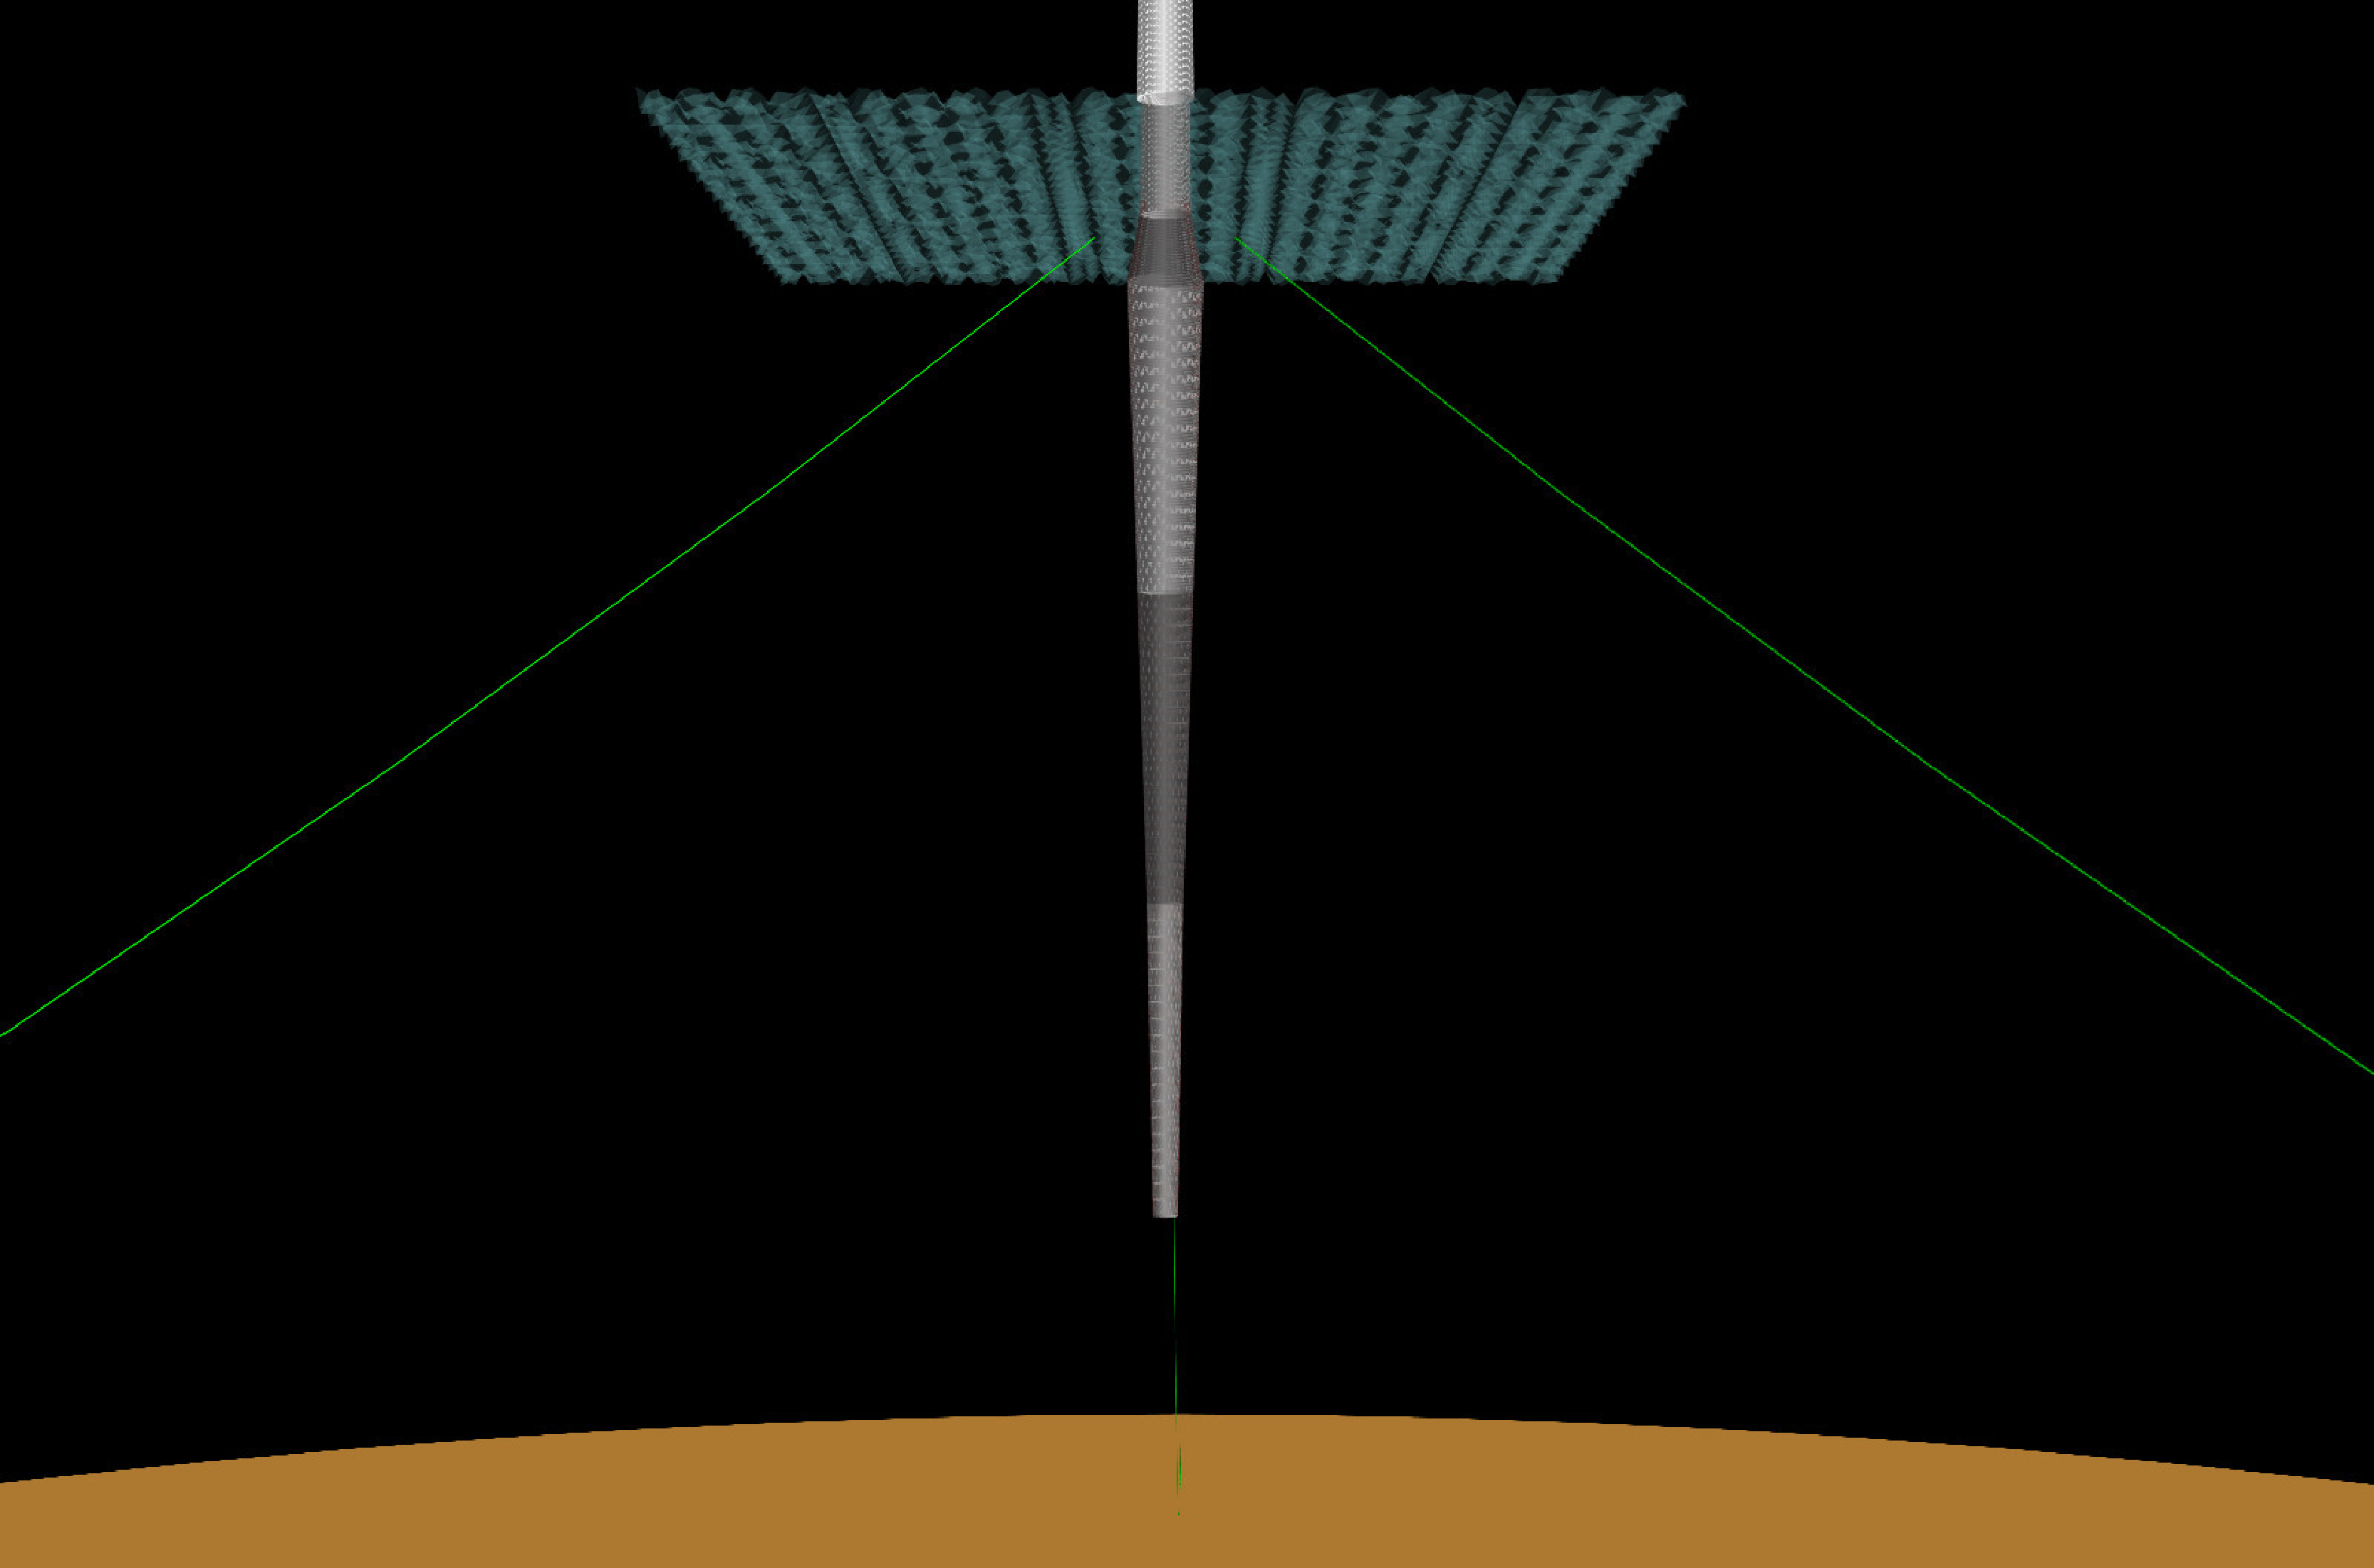
\includegraphics[width=\linewidth]{figs/spar-optimal.pdf}
    \caption{Spar}
  \end{subfigure}
  \begin{subfigure}[b]{0.49\linewidth}
    \centering 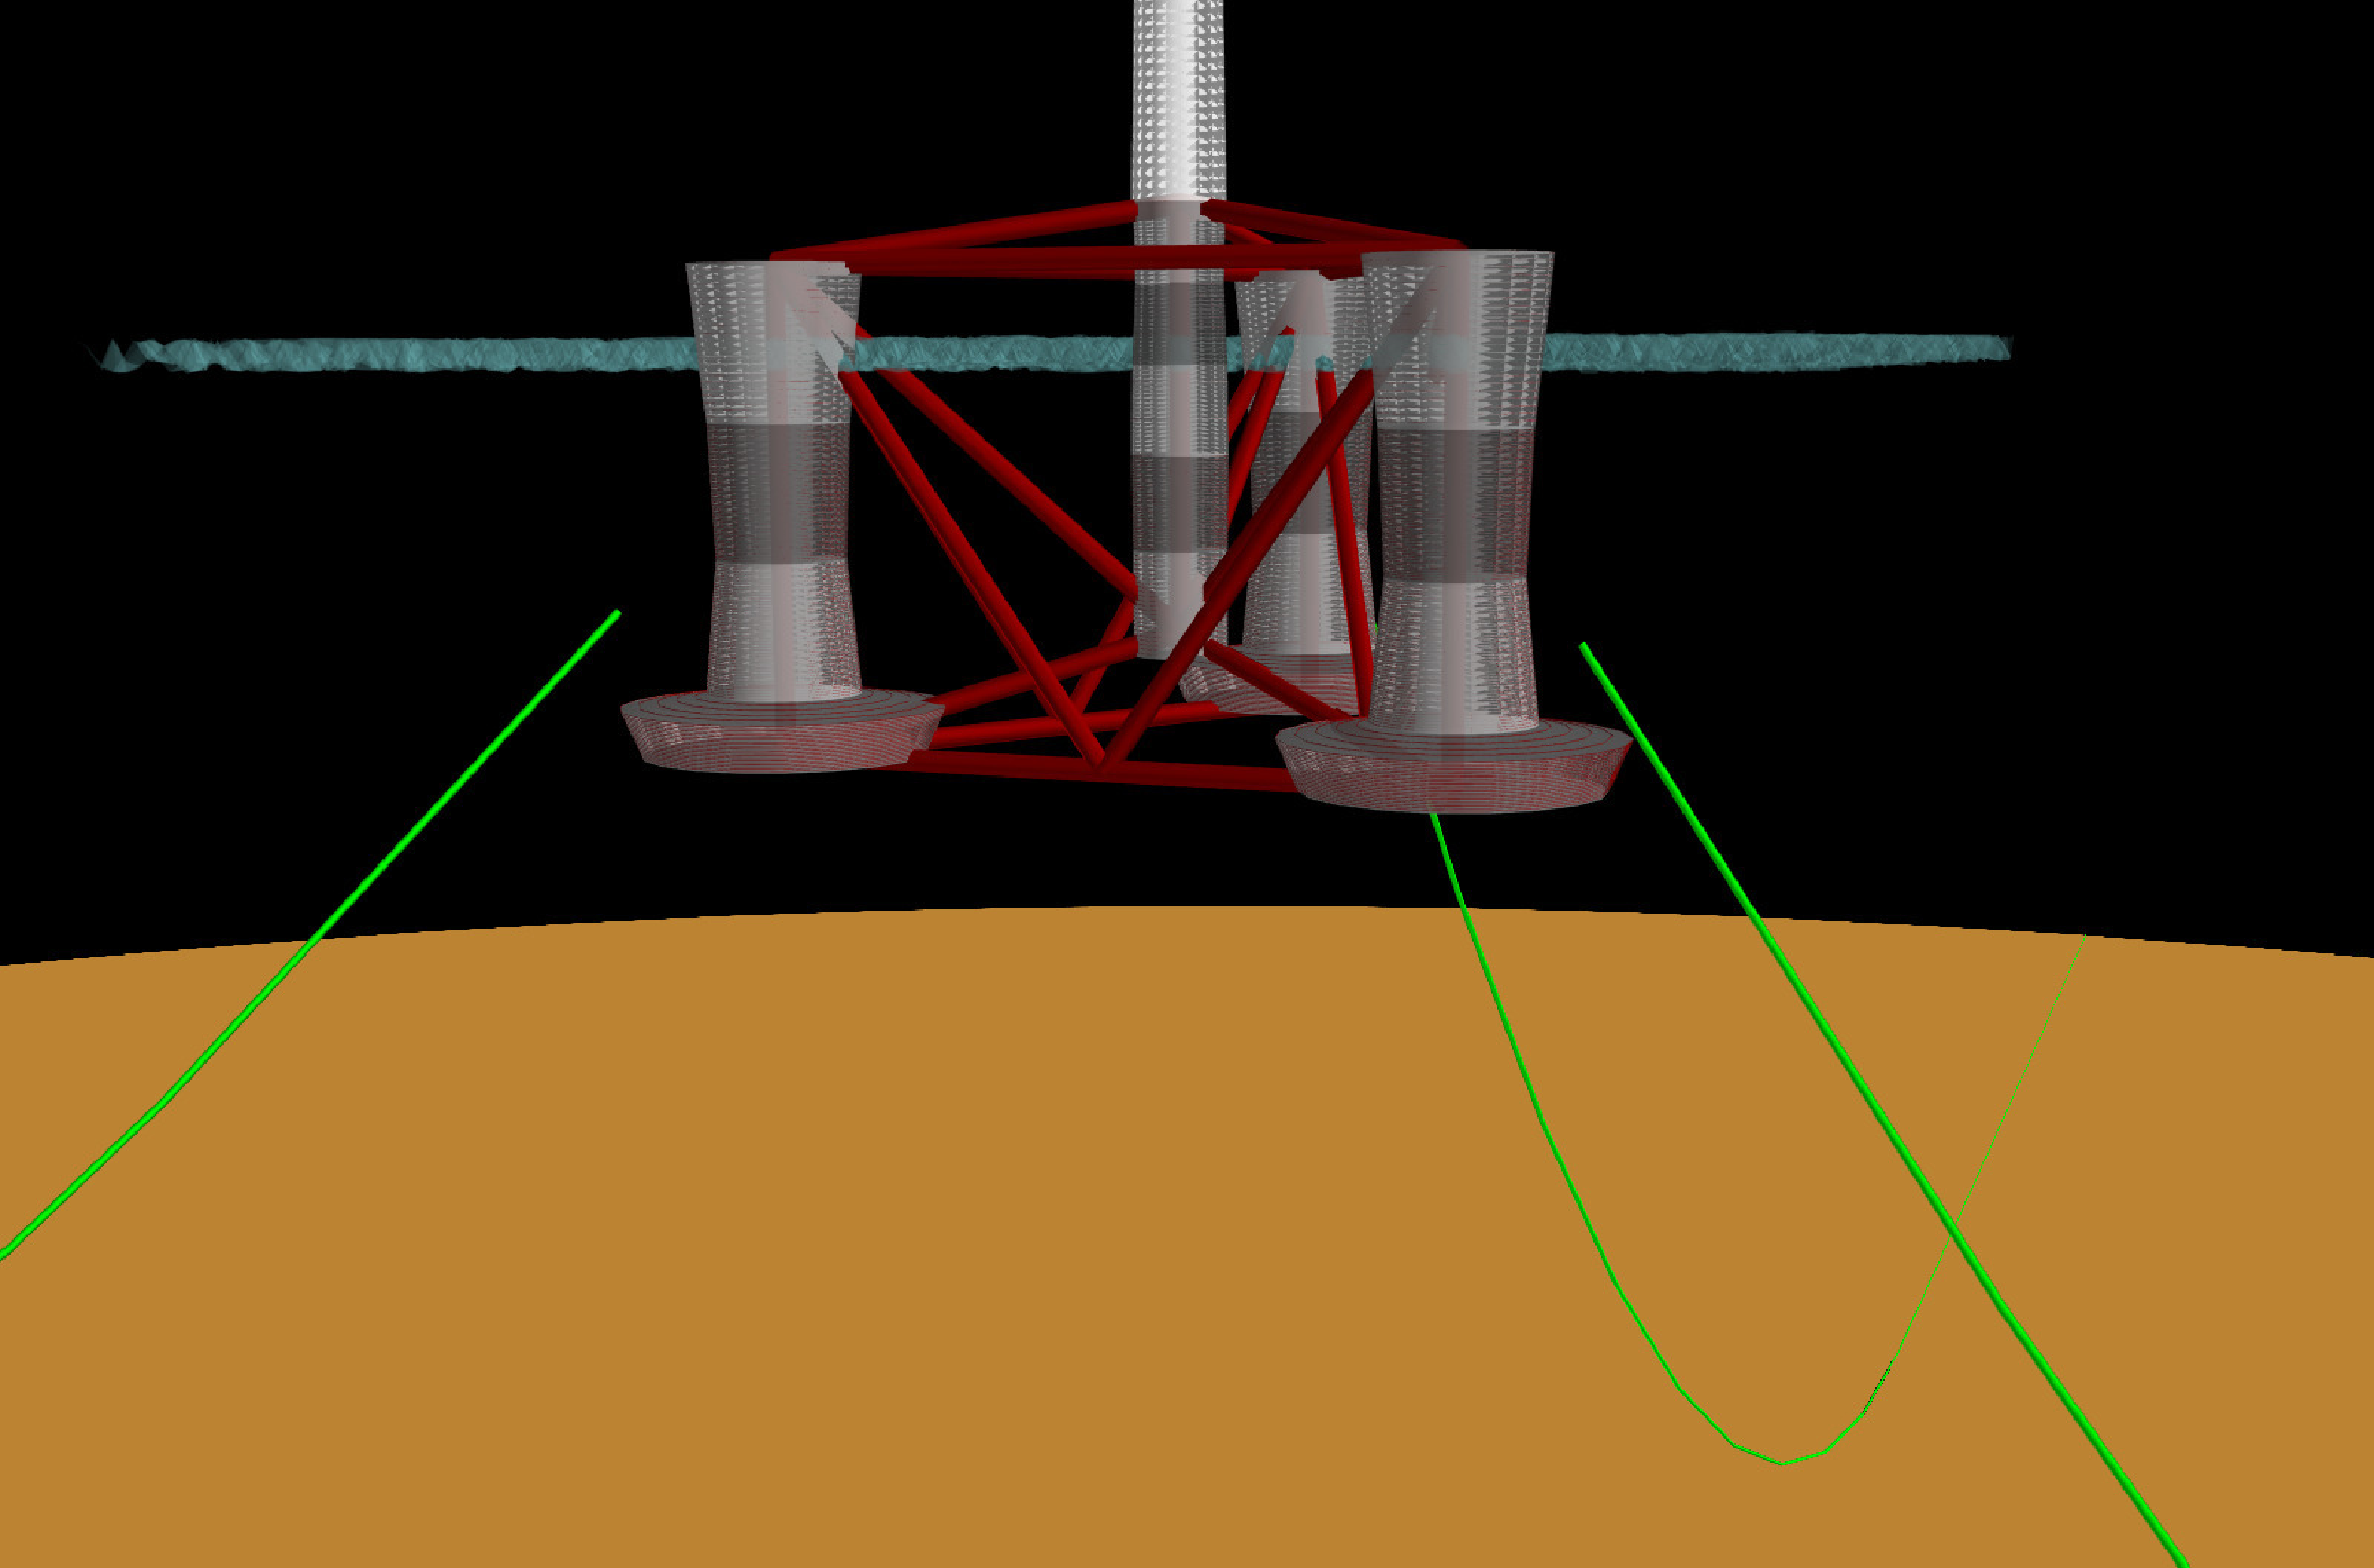
\includegraphics[width=\linewidth]{figs/semi-optimal.pdf}
    \caption{Semisubmersible}
  \end{subfigure}\\
  \caption{Examples of optimized spar and semisubmersible geometries.}
  \label{fig:optex}
\end{figure}



\chapter{WISDEM Floating Turbine Analysis}
\label{sec:other}
Direct WISDEM dependencies to \textit{CommonSE} and \textit{TowerSE}, as well as some of the
supporting utilities housed under the WISDEM umbrella, were mentioned in
Section \ref{sec:package}.  There are other inputs into \textit{FloatingSE} that
are outputs of other WISDEM modules.  For example force, moment, and
mass properties of the RNA.  An OpenMDAO Group that links these other
modules together to form a virtual floating turbine does not explicitly
fit within the conceptual boundaries of the \texttt{src/floatingse} package.
However, two files within the \textit{WISDEM} module (meant for
high-level coupling of multiple WISDEM components) \texttt{src/floating}-directory
do assemble the virtual floating turbine,

{\small
\begin{tabularx}{\textwidth}{ l X }
\texttt{floating\_turbine\_assembly.py} & OpenMDAO Group that connects  multiple WISDEM modules for a complete floating offshore turbine simulation and optimization.\\
\texttt{floating\_turbine\_instance.py} & Implements the above assembly
and extends.
\end{tabularx}
}

The WISDEM modules that exchange inputs and outputs within this
high-level assembly to crteate a virtual floating wind turbine are
listed in Table \ref{tbl:new_wisdem}.  In addition to
\textit{FloatingSE}, two other new WISDEM modules are also required to
fully represent a floating offshore wind plant (beyond just a single
turbine), \textit{OffshoreBOS\_SE} and \textit{Offshore\_OandM\_SE}.
With these two additions, WISDEM can be diagrammed as shown in Figure
\ref{fig:new_wisdem}.  While the core development of
\textit{OffshoreBOS\_SE} is effectively complete,
\textit{Offshore\_OandM\_SE} has not yet been implemented. Note that as
of this writing, \textit{DriveSE} is not yet connected to the others,
but doing so is part of the near-term development plan.

\begin{table}[htbp] \begin{center}
    \caption{WISDEM modules that comprise a virtual floating offshore
      wind plant.}
    \label{tbl:new_wisdem}
{\footnotesize
  \begin{tabularx}{\textwidth}{ l X } \hline
    \textbf{Module} & \textbf{Description} \\
\textit{RotorSE} & Analysis of aerodynamic and structural loading of rotor
  blades, determination of turbine power curve, and calculation of
  annual energy production (AEP)\\
\textit{CommonSE} & Wind and wave velocity profiles, drag calculations,
  probabilities distributions, frustum and tubular mass properties, math
  utilities, structural code compliance checks, and RNA aggregator\\
\textit{OffshoreBOS\_SE} & Capital costs for wind plant items aside from the
  turbine, such as cabling and substations.  Assembly, installation,
  commissioning, decommissioning, and financing costs for all
  components. See \citep{obos}\\
\textit{FloatingSE} & Floating substructure, including mooring and anchors, and
  static stability calculations\\
\textit{TurbineCostsSE (2015)} & Capital costs for all turbine components
  above the water line\\
\textit{PlantFinanceSE} & Roll-up of capital costs, balance of station
  costs, operational costs, financing rates, and net energy production
  into the levelized cost of energy (LCOE)\\
\textit{DriveSE} & Analysis of drive shaft, bearings, and gearbox.  See
  \citep{DriveSE}. NOT YET IMPLEMENTED\\
\textit{Offshore\_OandM\_SE} & Operational and maintenance costs.  NOT YET
    DEVELOPED\\
  \hline \end{tabularx}
}
\end{center} \end{table}

\begin{figure}[htb]
  \begin{center}
    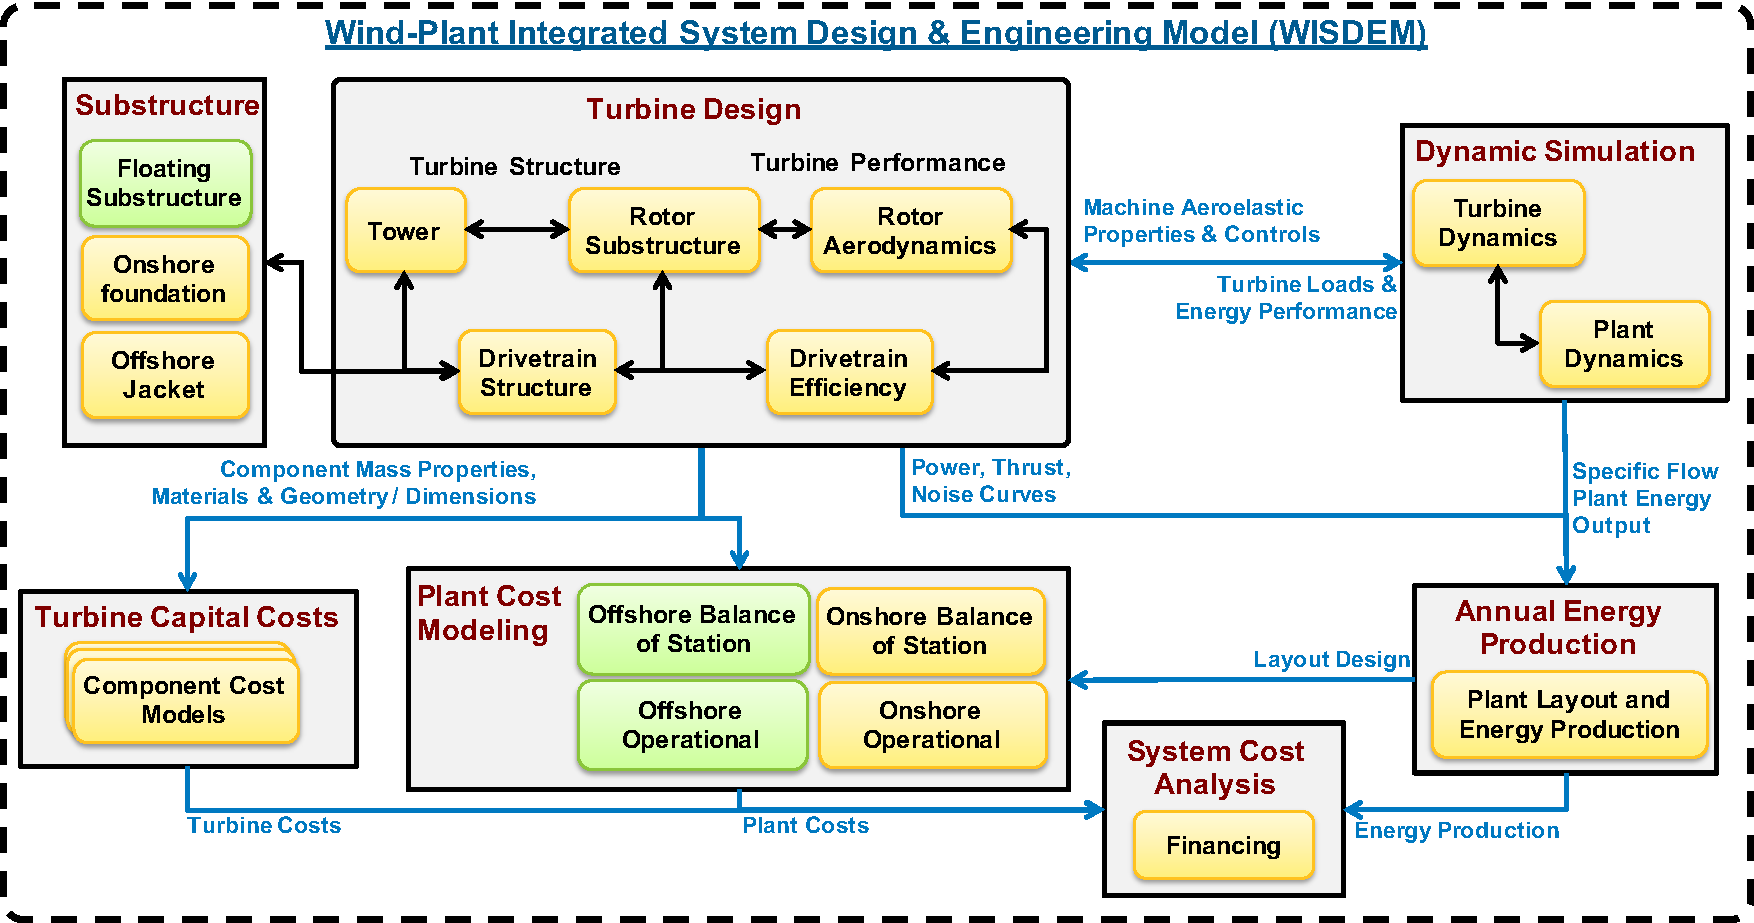
\includegraphics[width=6in]{figs/new_wisdem.pdf}
    \caption{Conceptual diagram of WISDEM following the addition of
      \textit{FloatingSE} and other modules (green boxes) to support offshore floating
      wind turbines.}
    \label{fig:new_wisdem}
  \end{center}
\end{figure}


With a floating offshore turbine constructed, system-wide optimization
and sensitivity studies can be conducted.  An obvious objective function
for these optimizations would be the levelized cost of energy (LCOE) as
output from the \textit{PlantFinanceSE} module.  This optimization would
require additional constraints pertinent to the other modules to produce
relevant results.  These other constraints are more suitably discussed
within the documentation of their home modules.  Depending on the nature
of the analysis, the user may wish to include other design variables in
the optimization that are inputs to one of these other modules.  As with
the constraints, the documentation of these design variables is best
found in their home modules.

%\section{Example}
%TODO

\begin{table}[htbp] \begin{center}
    \caption{Additional constraints used in full floating offshore
      turbine optimization.}
    \label{tbl:constraints-turb}
    {\footnotesize
  \begin{tabular}{ c l c l} \hline
    \textbf{Lower} & \textbf{Name} & \textbf{Upper} & \textbf{Description}\\
\hline \hline
    & \textbf{Rotor} &  &\\
 & rotor.P1\_margin & 1.00 & Blade frequency keep away from 1P rotor frequency\\
 & rotor.Pn\_margin & 1.00 & Blade frequency keep away from 3P rotor frequency\\
 & rotor.rotor\_buckling\_sparL & 1.00 & Rotor blade upper spar cap structural buckling unity constraint\\
 & rotor.rotor\_buckling\_sparU & 1.00 & Rotor blade lower spar cap structural buckling unity constraint\\
 & rotor.rotor\_buckling\_teL & 1.00 & Rotor blade upper trailing edge panel structural buckling unity constraint\\
 & rotor.rotor\_buckling\_teU & 1.00 & Rotor blade lower trailing edge panel structural buckling unity constraint\\
 & rotor.rotor\_damage\_sparL & 0.00 & Rotor blade upper spar cap structural damage constraint\\
 & rotor.rotor\_damage\_sparU & 0.00 & Rotor blade lower spar cap structural damage constraint\\
 & rotor.rotor\_damage\_teL & 0.00 & Rotor blade upper trailing edge panel structural damage constraint\\
 & rotor.rotor\_damage\_teU & 0.00 & Rotor blade lower trailing edge panel structural damage constraint\\
 & rotor.rotor\_strain\_sparL & 1.00 & Rotor blade upper spar cap structural strain unity constraint\\
  -1.00 & rotor.rotor\_strain\_sparU &  & Rotor blade lower spar cap structural strain unity constraint\\
 & rotor.rotor\_strain\_teL & 1.00 & Rotor blade upper trailing edge panel structural strain unity constraint\\
  -1.00 & rotor.rotor\_strain\_teU &  & Rotor blade lower trailing edge panel structural strain unity constraint\\
 & \textbf{Geometry} &  & \\
  20.00 & tcons.ground\_clearance &  & Minimum ground clearance of rotor blades\\
 & tcons.tip\_deflection\_ratio & 1.00 & Tip deflection limit to prevent tower strike as unity\\
 & \textbf{Stability} &  & \\
  1.00 & tcons.frequency1P\_margin\_high &  & Eigenfrequencies of entire structure must be below 1P frequency\\
 & tcons.frequency1P\_margin\_low & 1.00 & Eigenfrequencies of entire structure must be above 1P frequency\\
  1.00 & tcons.frequency3P\_margin\_high &  & Eigenfrequencies of entire structure must be below 3P frequency\\
 & tcons.frequency3P\_margin\_low & 1.00 & Eigenfrequencies of entire structure must be above 3P frequency\\
    \hline \end{tabular}
  }
\end{center} \end{table}


% bibliography
\cleardoublepage
\label{sec:Bib}
\printbibliography[heading=bibintoc]
\end{document}
